\documentclass[lineno]{jfm}

\usepackage{graphicx}
% \usepackage{epstopdf, epsfig}
\usepackage{newtxtext}
\usepackage{newtxmath}
\usepackage{natbib}
\usepackage{hyperref}
\hypersetup{
    colorlinks = true,
    urlcolor   = blue,
    citecolor  = black,
}
\newtheorem{lemma}{Lemma}
\newtheorem{corollary}{Corollary}
\newcommand{\RomanNumeralCaps}[1]
\linenumbers

\DeclareMathOperator{\Var}{\it Var}

\usepackage{pbox}
\usepackage{multirow}
\usepackage{color, colortbl}
\definecolor{Gray}{gray}{0.65}
\newcommand{\RowColor}{\rowcolor{} }

% \usepackage[final]{changes}
\usepackage[markup]{changes}
% \usepackage{mdframed}

\title{From convective to global instability in corrugated Couette-Poiseuille flow}

\author
{
 N. Yadav\aff{1} \and
 S. W. Gepner\aff{1} \corresp{\email{stanislaw.gepner@pw.edu.pl}}
}

\affiliation{\aff{1}Warsaw University of Technology, Institute of Aeronautics and Applied Mechanics, Nowowiejska 24, 00-665 Warsaw, Poland}

\begin{document}
\maketitle

\begin{abstract}
Couette-Poiseuille (CP) flow in the presence of longitudinal grooves is studied by means of numerical analysis. The flow is actuated by movement of the flat wall and pressure imposed in the opposite direction. Stationary wall features longitudinal grooves that modify the flow, change hydrodynamic drag on the driving wall and cause onset of hydrodynamic instability in the form of travelling waves with a consequent supercritical bifurcation, already at moderate ranges of the Reynolds number. We show that by manipulating this system it is possible to significantly decrease phase speed of the unstable wave and to effectively decouple timescales of wave propagation and amplification with a potential to change the character of the instability from convective to a global one. Current analysis begins with concise characterization of stationary, laminar CP flow and effects of applying selected corrugation pattern, followed by determination of conditions leading to the onset of linear destabilization. In the second part we illustrate selected nonlinear solutions obtained for low, supercritical values of the Reynolds numbers and due to the amplification of unstable travelling waves of possibly low phase velocities. The primary objective of this work is determination of flow conditions that lead to the onset of unstable modes and a consequent bifurcation of the solution into the nonlinear saturation state, characterized by possibly low advective speed of the secondary flow such that the distance traveled by the perturbation during amplification becomes small.
\end{abstract}

% \begin{keywords}
% hydrodynamic stability analysis, nonlinear solutions, Couette-Poiseuille flow, grooved geometry
% \end{keywords}

\section{Introduction}\label{sec:intro}
%% Do we need first two para
Use of patterned surfaces has been of interest as a potential method for passive control of various aspects of the flow.
Possible applications range from large-scale, turbulent flows, where surface manipulations have been investigated as means to reduce drag in the turbulent boundary layer \citep[i.e. riblets, see e.g.][]{luchini_manzo_pozzi_1991,goldstein_tuan_1998,jimenez2004turbulent},
down to small-scale, or even microfluidic arrangements as diverse as micro heat exchangers
for cooling of microelectronics, compact biochemical reactors or molecular and DNA screening devices \citep{Beebe2002}.
In the case of small-scale flows, enhancement of the diffusive transport \citep[see][for an extensive review]{Aref2017} along with low energy requirement is often the objective of the design, made especially difficult to achieve due to the fact that dynamics of such flows remains dominated by viscous effects \citep{Webb1983, Gepner2020b}.
In such cases patterned surfaces might be used in order to force enough complexity into the, otherwise laminar flow, causing onset of {\it chaotic advection} \citep{Aref1984, Aref2017} and resulting in sufficient kinematic stirring to significantly improve transport processes \citep{Stroock2002, Stremler2004}.

% While number of possible surface patterns is limit-less, here we focus on the large-scale wall roughness in the form of longitudinal grooves (see figure \ref{fig:longitudinal_groove}), such that lines of constant elevation remain parallel to the streamwise direction.
% Up to date, an alternative configuration, consisting of unidirectional grooves, oriented transversely (such that ridges run perpendicular to the flow) to the streamwise direction received more attention.
% The interest in this problem can be traced back to the work of \citet{Sobey1980a} and experimental investigations by \citet{Nishimura1984,Nishimura1985,Nishimura1990b,Nishimura1990a}.
% Two types of unstable modes have been identified for this configuration.
% The first one is a shear-driven travelling wave \citep{Blancher1998,Floryan2010,Cabal2002,gepner2016flow, Rivera2013}, similar to the classical Tollmien-Schlichting (TS) wave of the plane Poiseuille flow.
% The second unstable mode is attributed to centrifugal forces associated with groove-imposed changes of the stream direction and has a form of streamwise vortices that remain stationary with respect to the surface pattern.
% This mode connects in the smooth channel limit to a stationary Squire has been shown to play a critical role in channels with a certain class of grooves \citep{Floryan2010,gepner2016flow}.
% Also, its existence has been documented experimentally by \citet{Gschwind1995,mitsudharmadi2012},
% and through numerical simulations by \citet{Cho1998,Cabal2002,Floryan2003,Floryan2005}.
%% Do we need first two para

%% Why not start here?

\begin{figure}
\centering
	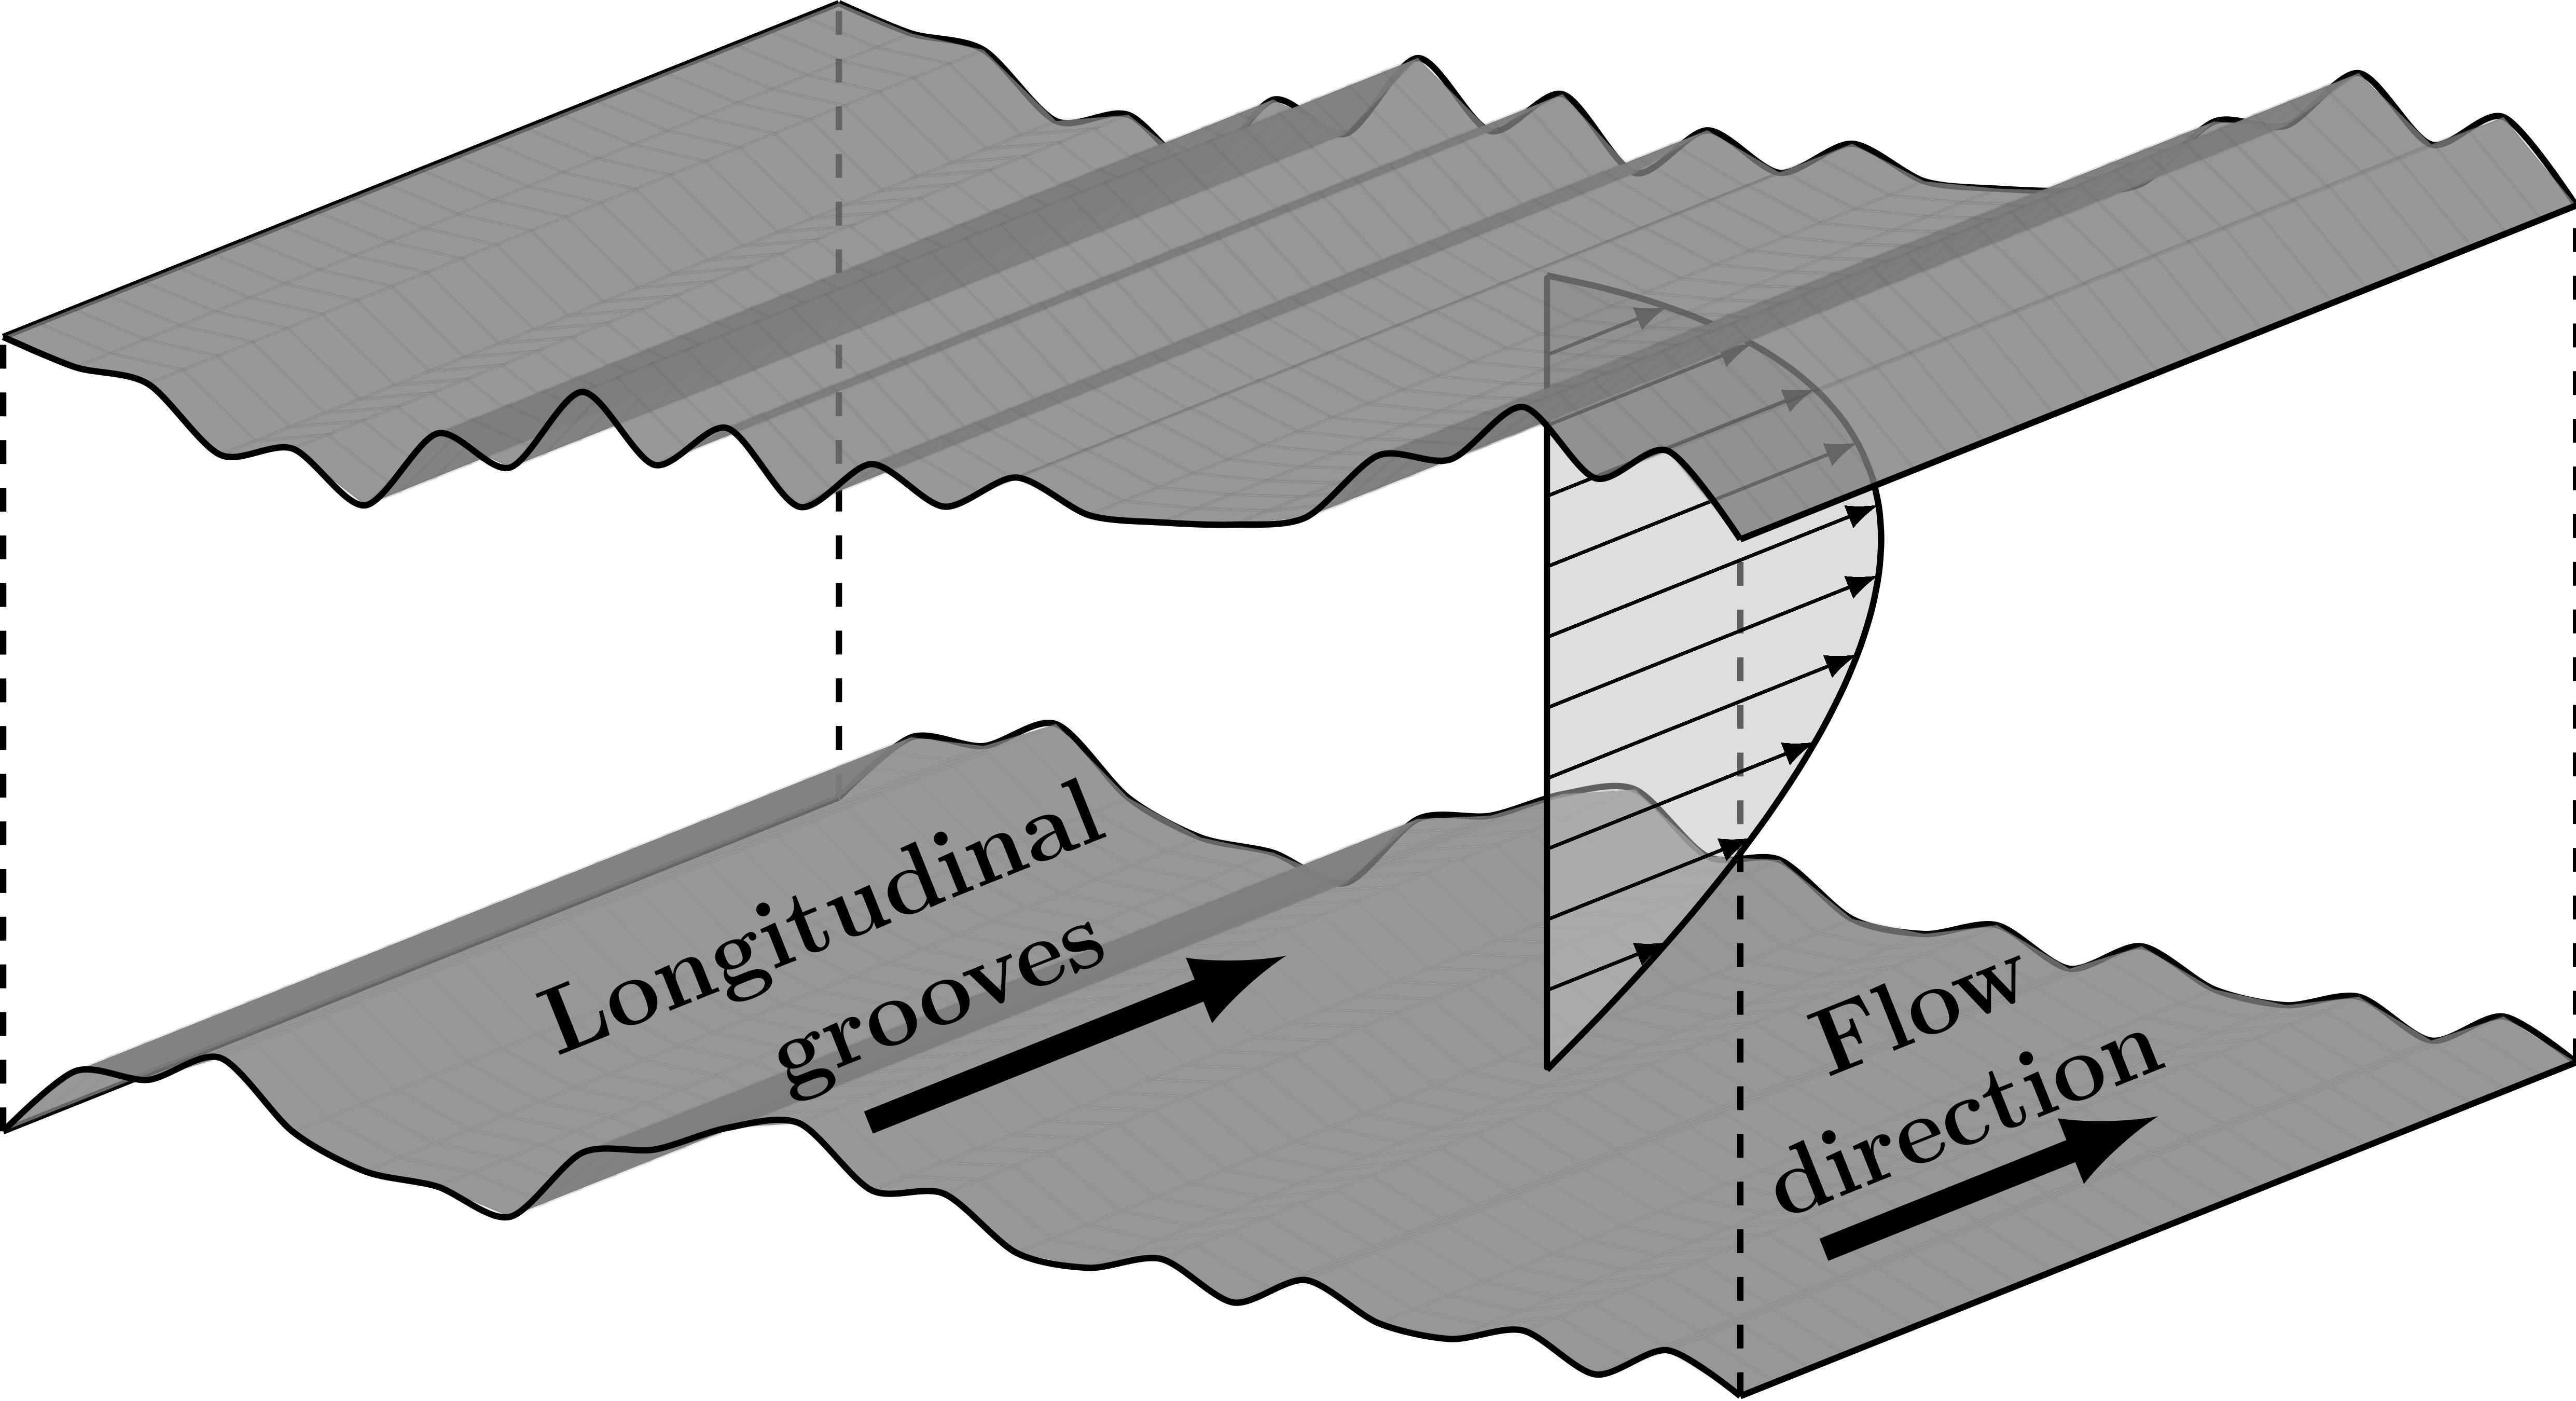
\includegraphics[width=0.55\textwidth]{long_groove.png}  
	\caption{Longitudinal grooves.}
	\label{fig:longitudinal_groove}
\end{figure}

While number of possible surface patterns is limit-less, here we focus on the 
regular wall roughness in the form of longitudinal grooves positioned such that ridges of the geometry run parallel to the flow direction, as schematically illustrated in Figure \ref{fig:longitudinal_groove}.
This type of grooves has been investigated as a mean to manipulate flow dynamics in doubly-periodic grooved channel \citep{Szumbar2007, mohammadi2014effects, Mohammadi2015, Nikesh2017, Gepner2020, Gepner2020b}, singly-periodic corrugated duct \citep{Nikesh2018, Pushenko2021} and grooved, annular \citep{moradi2019flow, moradi2019drag} configurations.
It has been shown that properly shaped longitudinal grooves lead to reduction of hydraulic drag \citep{Szumbar2011, szumbarski2011impact, mohammadi2015numerical, Ng2018, moradi2019drag}.
Interestingly, there are indications, both experimental \citep{Bolognesi2014,Kim2012} and theoretical \citep{crowdy2017},
that drag reduction, attributed to super-hydrophobic effect could, at least in some cases be related to drag reduction reported for flows through longitudinally patterned geometries, such as those considered here.

Longitudinal grooves introduce variation of the streamwise velocity component and have been shown to result in the onset of two types of instabilities.
The first is shear driven, similar to the classical Tollmien-Schlichting (TS) wave of the plane Poiseuille flow and has been described in detail by \citet{moradi2014stability}.
The second is inviscid in nature and results from deformation of the spanwise distribution of the streamwise velocity component that results from the presence of longitudinal grooves.
This mechanism has been reported by \citet{Szumbar2007} and described in detail by \citet{Mohammadi2015,Nikesh2017}.
This mode has a form of a wave travelling downstream and becomes amplified at Reynolds numbers that are two orders of magnitude lower than those established for the onset of a TS wave in the case of plane Poiseuille flow (canonical plane channel flow linear stability limit of approximately $Re=5772$, using channel's half height and maximum laminar, centre-line velocity as scales), and much below the sub-critical transition limits reported for the case of plane channel flow \citep{carlson1982flow, Gome2020} of slightly below $Re=1000$.
In this work we consider the second, inviscid instability mechanism.

While numerical investigations characterizing effects of longitudinal corrugation on hydrodynamic stability \citep{Szumbar2007, Szumbar2011, Mohammadi2015}, and analysis of consequent nonlinear states \citep{Nikesh2017,Pushenko2021} have been performed, to this date there seem to be no experimental results reported to support existing numerical findings.
The lack of experimental results is somewhat surprising, considering that the alternative, transverse groove configuration received much attention, both from experimental as well as computational perspectives \citep[][]{Sobey1980a,Nishimura1984,Nishimura1985,Nishimura1990b,Nishimura1990a,Gschwind1995,mitsudharmadi2012,Blancher1998,Floryan2010,Cabal2002, gepner2016, Rivera2013,gepner2016}.
On the other hand it seems that, at least in the qualitative sense, destabilization mechanism caused by the presence of longitudinal grooves and consequent variation in the streamwise velocity, is similar to the gap instability \citep{Gagnon_Tavoularis_2021, moradi2019flow} that exist in the eccentric annular flow configuration and has been experimentally investigated \citep{Piot2011}.

To the best of authors' knowledge shortage of experimental results for the case of longitudinal grooves is not for the lack of trying,
as experimental verification has been attempted by at least two groups.
The first effort comes form the work of \citet[][a PhD thesis in Polish]{Blonski2007},
where a micro-PIV setup was used to study effects of longitudinal grooves.
Results of this experiment were described in
\citep{szumbarski2011impact} but focus was given only to the drag reducing effect,
and characterization of hydrodynamic stability remained at best cursory.
The second attempt was carried out by the group that conducted successful experimental investigations for the case of transverse configurations \citep{Asai2006,Floryan2011}.
However, our understanding is that for the longitudinal configuration the effort undertaken by that group was not successful.%  \citep[][private communications]{Floryan_private_communications}.

One of the problems in conducting a successful experiment is the fact that considered instability is convective and has a form of a wave travelling downstream.
Such an unstable mode, if amplified, develops downstream at a relatively slow pace,
while all the time being advected with the speed that is comparable with the bulk flow velocity.
This, in turn, requires any prospective experimental set-up to imitate periodicity conditions, so easily enforced numerically,
either by resorting to the corrugated Taylor-Couette configuration \citep[see][for numerical analysis of such configuration]{Ng2018}
or by application of impractically long arrangements with very long test sections,
such as to allow for the development of the unstable mode long enough for it to become detectable.
Preferably measurement section should be long enough to the point where nonlinear interactions cause nonlinear saturation and onset of secondary flows, before bulk of the flow flushes the investigated phenomena out of the measurement domain.

A viable alternative might lie in manipulating the flow system in such a way as to decrease propagation speed of the unstable mode to the point that it can be considered a stationary one.
Ideally, such manipulation should result in the change of the instability character, at least during linear amplification phase, from convective to a global one.
We mean by that the fact, that during amplification of a sufficiently decelerated mode and while it remains small,
spacial growth of resulting secondary structures would manifest both up- as well as down-stream,
in contrast to the purely convective instability that amplifies only downstream.
Preferably such system manipulation would allow to maintain the low Reynolds number requirement for destabilization.
An interesting solution to this problem comes from application of the Couette-Poiseuille (CP) configuration with pressure applied to act opposite to the movement of the driving wall.
Such configuration, featuring very low or even zero-mean flow was proposed by \citet{Klotz_2017_prf} for the study of transitional turbulence.
It has been successfully applied to experimental investigation of transient amplification of turbulent spots \citep{Klotz_2017_jfm}, quenching experiment \citep{liu_klotz_2021} and measurements of large- and small-scale flows in planar CP flow configurations \citep{klotz2021experimental}, allowing for long time scales to be obtained in measurements.
The rationale for this solution comes from the fact that localized, turbulent features are advected with speeds comparable to the mean velocity of the base flow.
Thus, reducing this speed keeps them stationary in the laboratory frame of reference.
Similarly, the unstable mode that results from longitudinal corrugation, and which is of interest to this work, travels at a speed that is related to the mean velocity of the base flow.
In principle, sufficiently limiting propagation speed of this mode should allow for the qualitative change of the instability character from convective to global, with growth during the linear amplification stage propagating both up- as well as downstream.
Consequently, ensuing secondary flows might become stationary or at least slowly advected allowing for longer observation times to be possible using relatively compact experimental arrangements.

The main intention of the current work is to address the problem of hydrodynamic stability of the CP flow, modified with regular, longitudinal corrugation applied to the stationary wall.
Of primary interest is characterization of stability properties and determination of flow conditions that result in low Reynolds number ($Re<500$) destabilization of the flow and at the same time cause propagation speed of the unstable mode to become as low as possible,
preferably to the point that the instability may be treated as a global one with the ensuing secondary flow forming a slowly propagating or a standing wave like state.
To this end focus is given to configurations that lead to base flows characterized by zero-mean flow and low phase speed of the unstable mode (it turns out those two do not necessarily lead to the same conditions). 
At last, this paper addresses a conjecture which states that the form of the instability detected for the case of corrugated Poiseuille flow \citep{Nikesh2017} is also attainable in the Couette configuration
% \citep[][private communications]{Floryan_private_communications},
an issue that, surprisingly remains uninvestigated today.

The layout of this paper is as follows. In $\S$\ref{sec:problemDes}, we formulate the flow problem, define geometry, and discuss the computational approach used in this work. In $\S$\ref{sec:2dflow} properties of the base flow are discussed and zero-mean flow conditions are selected and characterized.
In $\S$\ref{sec:linearStability} hydrodynamic stability for the corrugated CP flow is provided.
Possible decrease in phase velocity of the unstable wave mode is discussed and suitable conditions selected for further analysis.
Section $\S$\ref{sec:nonlinear_saturation} describes Direct Numerical Simulation (DNS) at supercritical flow conditions performed for cases corresponding to zero-mean stationary flow and those that significantly limit propagation speed of the unstable mode.
Section $\S$\ref{sec:conclusion} concludes the work and provides a brief summary.

\section{Problem Description}\label{sec:problemDes}
Consider flow of an incompressible, Newtonian fluid through a channel with a plane top and corrugated bottom wall schematically illustrated in Figure \ref{fig:geom1}.
The channel is assumed to be doubly periodic in the streamwise $z$- and spanwise $x$-direction and constrained by walls located at:
\begin{equation}
\begin{cases}
y_{u} = 1,  \\
y_{l}= -1 + S\cdot cos(\alpha x),
\end{cases}
\label{eq:wall}
\end{equation}
with $\alpha$ and $S$ the corrugation wave number and amplitude. The resulting groove pattern runs parallel to the streamwise $z$-direction.

 \begin{figure}
 \centering
 	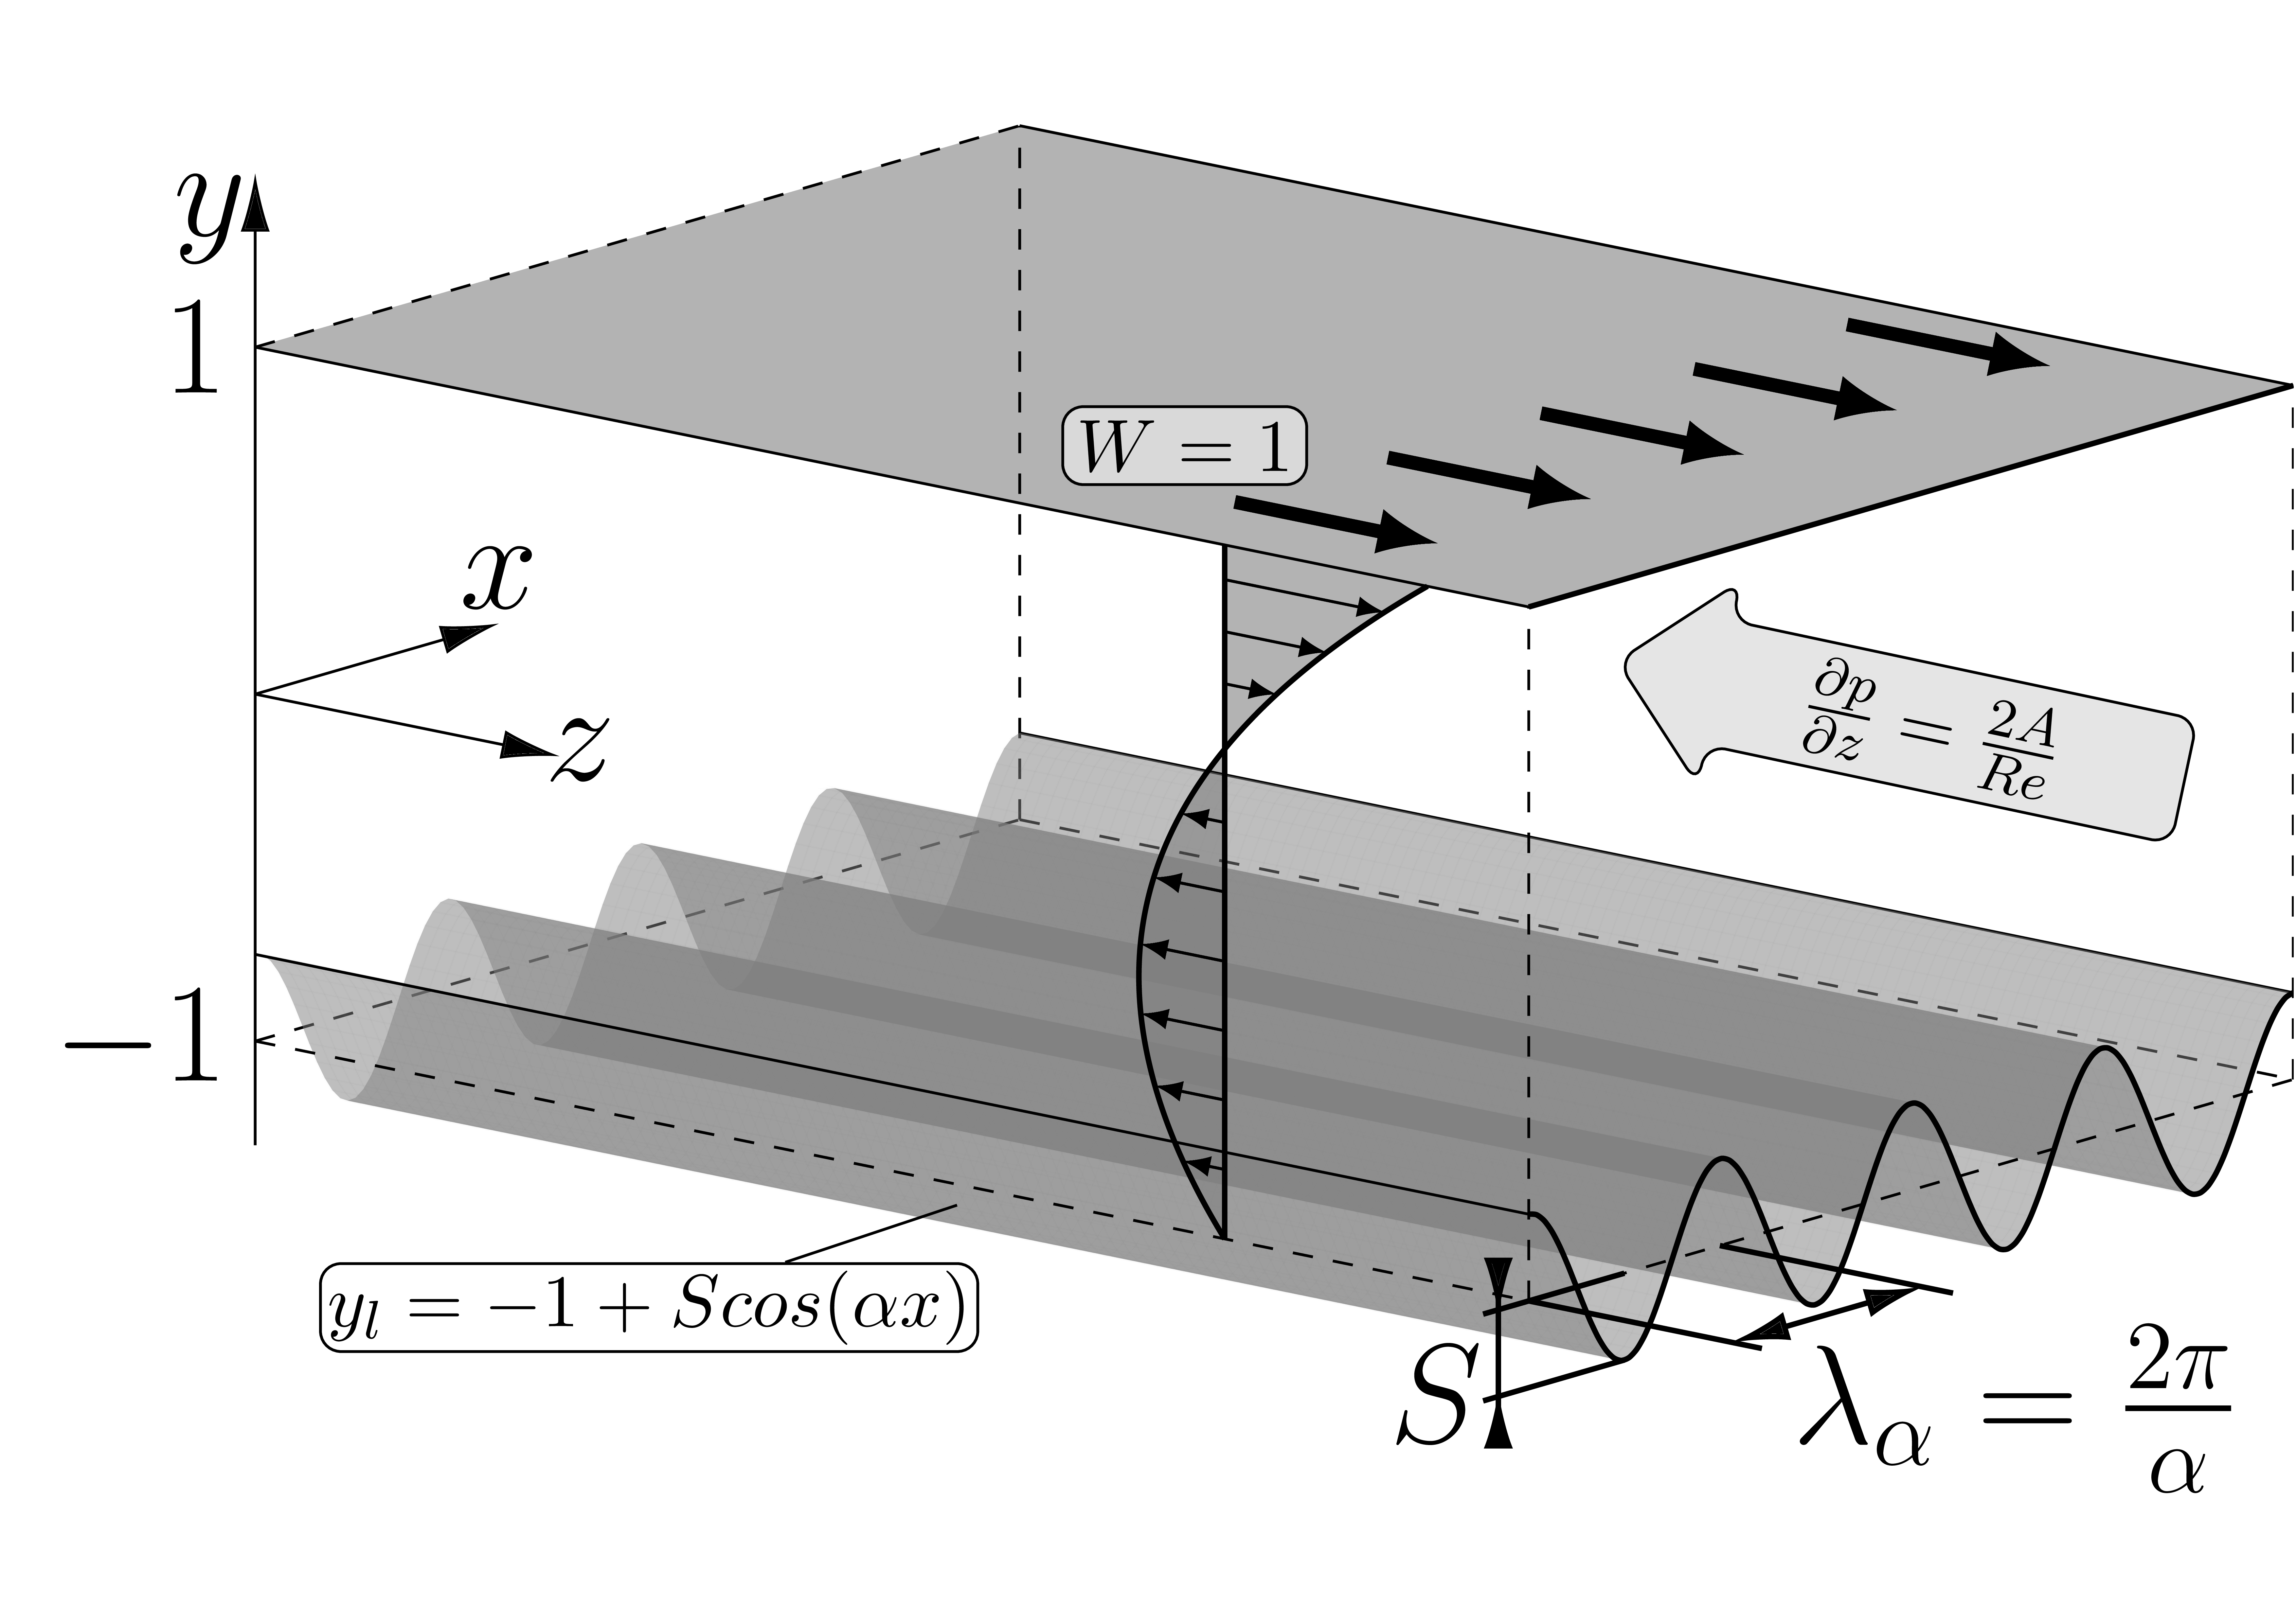
\includegraphics[width=0.85\textwidth]{geom.png}  
 	\caption{Channel geometry.}
 	\label{fig:geom1}
 \end{figure}

The flow is driven by motion of the plane, top wall towards positive $z$-direction (the Couette component) and pressure applied to act in opposition (the Poiseuille component) with the corrugated, bottom wall remaining stationary.
Half of the average distance $h$ between walls defines the length scale and velocity $W$ of the moving top wall is used as the velocity scale.
Time is scaled with ${h}/{W}$, pressure with $\rho W^2$ where $\rho$ stands for density and is taken to be a unit.
Reynolds number corresponding to the Couette component is $Re={W h}/{\nu}$ where $\nu$ denotes kinematic viscosity.
Applied pressure is $p=2A z/Re$ and acts against motion of the top wall with $A$ representing the Poiseuille pressure ratio parameter.
We note that pressure ratio is selected such that in the absence of the Couette component for the smooth channel case ($S=0$), $A=1$ results in parabolic profile with the centre line velocity $W_p=-1$.
Consequently the Poiseuille component Reynolds number is $Re_p=A Re$.
The flow velocity vector field ${\bf u}=[u, v, w]^T$ satisfies continuity and momentum equations, that can be written as:
\begin{equation}
\begin{cases}
\nabla \cdot {\bf u} = 0,\\
\frac{\partial {\bf u}}{\partial t} + ({\bf u} \cdot \nabla){\bf u} = -\nabla p + \frac{1}{Re} \nabla^2 u + {\bf f},\\
\end{cases}
\label{eq:NS}
\end{equation}
where $\bf f$ represents forcing used to excite
unstable modes in the stability and nonlinear analysis, and otherwise is taken to be zero.
The flow problem is augmented with appropriate boundary conditions imposed at the top and bottom wall
along with periodicity conditions in the streamwise and spanwise directions,
and of the form:
\begin{equation}
\begin{cases}
{\bf u} = [0, 0, 1]^T\text{ at } y=y_{u},\\
{\bf u} = [0, 0, 0]^T \text{ at } y=y_{l},\\
{\bf u}(x=0)={\bf u}(x=kL_x) \text{ for } k=\pm1,\pm2, \text{...},\\
{\bf u}(z=0)={\bf u}(z=mL_z) \text{ for } m=\pm1,\pm2, \text{...},
\end{cases}
\end{equation}
with $L_x$ and $L_z$, dimensions of the computational domain in the periodic directions.
Irrespective of the corrugation amplitude, under constant pressure gradient aligned with the geometry there exist a stationary, laminar solution that is streamwise invariant.
This reduces \eqref{eq:NS} to a Poisson problem for streamwise velocity, of the form:
\begin{equation}
    \Delta w = 2A,
    \text{ with }
    \begin{cases}
    w=1\text{ at }y=y_{u}\\
    w=0\text{ at }y=y_{l}\\
    w(x=0)=w(x=kL_x) \text{ for } k=\pm1,\pm2, \text{... .}
    \end{cases}
    \label{eq:poiss}
\end{equation}
Consequently the resulting velocity vector for the stationary, laminar flow is \begin{equation}
    {\bf U}(x,y) = [0, 0, w(x,y)].
    \label{eq:laminar_solution}
\end{equation}

In the forthcoming analysis we shall maintain the Couette component fixed, and manipulate pressure ratio of the Poiseuille component $A$, such as to minimize either the bulk velocity of the laminar flow, or phase speed of the occurring unstable mode.
For the case of zero amplitude corrugation, considered problem is identical to the plane CP configuration
and consequently, primary reference is the canonical Couette flow between infinite parallel plates placed at $y=\pm1$, driven by constant wall velocity, characterized by velocity vector field ${\bf u} = [0,0, 0.5(y+1)]$ and flow rate per unit width $\Dot{V}_c=1$.
The secondary reference is the Poiseuille flow in the opposite direction and characterized by ${\bf u} = [0,0, A(y^2-1)]$ with flow rate per unit width $\Dot{V}_p=-4A/3$, using the adopted Poiseuille pressure ratio parameter $A$.
In the case of plane channel flow, the resulting CP combination yields flow velocity ${\bf u} = [0, 0, A(y^2-1)+0.5(y+1)]$ with $A=0.75$ for the case of zero bulk flow \citep{Klotz_2017_prf, mohammadi2014effects}.
Corrugation of the stationary, bottom wall changes the laminar flow and the pressure ratio $A$ leading to the zero mean flow needs to be recalculated.

For the pressure driven flow presence of longitudinal grooves has been shown to cause onset of nonlinear flow solutions \citep{Nikesh2017,Nikesh2018,moradi2019flow}, to which the flow transitions via a supercritical Hopf bifurcation \citep{Gepner2020} already at very low values of the Reynolds number (critical conditions occur below $Re=60$ using the Poiseuille, centre-line velocity scale).
Those nonstationary solutions remain connected to the laminar state in the linear sense and are linked to the travelling wave mode instability that develops due to the corrugation induced variations in the streamwise velocity.
In this work, onset of secondary flows is addressed in two steps.
First, by means of modal, linear hydrodynamic stability theory with linearization of \eqref{eq:NS} around stationary, laminar flow solution \eqref{eq:laminar_solution}.
Second, by means of the DNS of flows at supercritical conditions and up to the onset of nonlinear interactions in the saturation process. 
For the linear part the flow is represented as a superposition of the stationary solution \eqref{eq:laminar_solution} $({\bf U}, P)$ and a small disturbance, i.e:
\begin{equation}
    \begin{cases}
        {\bf U}_T(x,y,z,t)={\bf U}(x,y)+{\bf u}_p(x,y,z,t), \\
        P_T(x,y,z,t)      = P(x,y)+p_p(x,y,z,t),
    \end{cases}
    \label{eq:total}
\end{equation}
where subscripts $T$ and $p$ stand for total and perturbation quantities.
Perturbed quantities \eqref{eq:total} are substituted into governing equations \eqref{eq:NS}, followed by standard linearization of the perturbation problem.
Form of the perturbation is restricted to a normal mode, periodic in the spanwise $x$- and streamwise $z$-direction, of the form:
\begin{equation}
    \begin{cases}
        {\bf u_p}(x,y,z,t)={\bf \widehat{u}}_p(x,y)e^{i(\beta z + \delta x - \sigma t)}+{\it c.c.}, \\
        p_p(x,y,z,t) = \widehat{p}_p(x,y)e^{i(\beta z + \delta x - \sigma t)}+{\it c.c.},
    \end{cases}
    \label{eq:normal_mode}
\end{equation}
where ${\bf \widehat{u}}_p$ and $\widehat{p}_p(x,y)$ are perturbation amplitude functions, \textit{c.c.} stands for complex conjugate, $(\beta, \delta)$-pair represents the streamwise and spanwise wave numbers (treated as parameters) and $\sigma=\sigma_r+i\sigma_i$ is the complex amplification rate whose real and imaginary parts correspond to perturbation frequency and growth rate, respectively.
We note that \citet{Nikesh2017} shows that within the linear range and at moderately supercritical conditions, for the considered type of instability the spanwise
periodicity of the mode, characterized by the wave number $\delta$ (see \eqref{eq:normal_mode}) is bound to the periodicity of the corrugation pattern, characterized by geometrical wave number $\alpha$ (see \eqref{eq:wall}), i.e. $\delta=\alpha$, with the streamwise wave number $\beta$ remaining a parameter.
The linearized flow problem with perturbation \eqref{eq:normal_mode} leads to a generalised eigenvalue problem for the partial differential equations for the modal functions with $\sigma$ as the complex eigenvalue.
Discretization transforms this problem into an algebraic eigenvalue problem for $\sigma$
% , of the form:
% \begin{equation}
%     A{\bf u}_j = \sigma_j{\bf u}_j
%     \label{eq:eigen_system}
% \end{equation}
which is solved numerically.

In the forthcoming analysis the arising flow and stability problems are solved using the spectral element/hp solver available within Nektar++ software package \citep{Cantwell2015}.
Spatial discretization is based on spectral element discretization in the spanwise $(x,y)$ plane augmented with Fourier’s decomposition in the streamwise $z$-direction, truncated to $M$ leading modes and of the form:
\begin{equation}\label{eq:modes}
    \textbf{u}(x,y,z,t) =   \sum_{k=-M}^{k=M} {\bf u}_k e^{ik\beta z}
\end{equation}
with conjugacy condition {${\bf u}_k={\bf u}^*_{-k}$}.
Spectral element grid spans the $(x,y)$ plane and uses structured quadrilateral
mesh of $13\times11$ elements per corrugation section, generated with the GMSH package \citep{GMSH2009}.
Within each mesh element local polynomial expansion is performed with a modified Jacobi base \citep{Cantwell2011}
consisting of hierarchical assembly of
$6$, up to the $5$'th order polynomials,
combined with Gauss-Lobatto-Legendre quadrature using $6$ quadrature points, in each elemental direction.
The number of Fourier modes used in expansion \eqref{eq:modes} for calculation of the nonlinear states is selected such that ratio of the modal energy of the leading, $0$'th mode (the mean flow), to the $M$'th (highest used in calculations) mode is sufficiently large.
Temporal discretization is achieved with the second-order velocity-correction scheme \citep{Serson2016velocitycorrection}.
Spatial accuracy of the computational approach used here is verified by resolving the demanding hydrodynamic stability eigenproblem on a sequence of meshes and with varying polynomial expansion order. Results of this verification are outlined in the Appendix. We also note that the approach used here has already been established for similar flows \citep{gepner2016,Nikesh2017,Nikesh2018,Nikesh2021,Hossain2021spectral} and both spatial and temporal resolutions used in this work are more than sufficient to recover both hydrodynamic stability and nonlinear saturation states, as outlined in \cite{Nikesh2017}.

In the remainder of this work we shall concentrate on a single corrugation pattern, characterized by corrugation wave number and amplitude pair $(\alpha, S)=(1,0.7)$.
Focus will be given to the influence of pressure ratio $A$ of the Poiseuille component on hydrodynamic stability, propagation speed of the unstable wave and character of the resulting secondary flows with interest in deceleration of the nonlinear flow pattern resulting from amplification of the unstable wave mode.
This choice of the geometrical configuration is dictated by the fact that this geometry results in amplification of the travelling wave mode instability already at values of the Reynolds number that are close to the lowest available (below $60$), at the same time offers drag reduction in the case of pressure only driven flow \citep{Gepner2020b, Nikesh2017} and allows to achieve significant decrease of the unstable wave propagation speed at moderate and low values of the Reynolds number ($Re<500$).

%%%%%%%%%%%%%%%%%%%%%%%%%%%%%%%%%%%%%%%%%%%%%%%%%%%%%%%%%%%%%%%%%%%
%%%%%%%%%%%%%%%%%%%%%%%%%%%%%%%%%%%%%%%%%%%%%%%%%%%%%%%%%%%%%%%%%%%

\section{Stationary flow solution}\label{sec:2dflow}
\begin{figure}
\centering
 \includegraphics[width=0.85\textwidth]{A075_velocity_contour.pdf}  
 \caption{Contours of the streamwise velocity component of the stationary solution for a single corrugation section characterized by $(\alpha,S)=(1,0.7)$ (left) compared to the plane CP flow (right) for pressure ratio $A=0.75$. Solid line distinguishes $w=0$ contour.}
 \label{fig:streamwise_vel}
\end{figure}

\begin{figure}
\centering
 \includegraphics[width=0.85\textwidth]{A075_velocity_profile.pdf}  
 \caption{Streamwise velocity profiles of the stationary solution at $x/\lambda_\alpha=0, 0.25, 0.5$ (left) compared to the plane CP flow (right). Conditions same as in figure \ref{fig:streamwise_vel}.}
 \label{fig:streamwise_prof}
\end{figure}

Detailed characterization of stationary, laminar CP flow in the presence of wall corrugation has already been provided by \citet{mohammadi2014effects}. The analysis contained therein has been performed for a wide range of geometries, both by means of semi-analytical asymptotic analysis and domain transformation based numerical method.
In the case of a stationary, plane CP flow it remains invariant in the spanwise direction, satisfies \eqref{eq:poiss} and at $A=0.75$ features zero mean flow rate.
Imposition of grooves introduces spanwise variation of the streamwise component and modifies the stationary flow.
For $A=0.75$ this change is illustrated in figures \ref{fig:streamwise_vel} and \ref{fig:streamwise_prof} by means of contours and profiles of streamwise velocity,
both for the corrugated and reference, plane CP flow.
The most prominent change due to the imposition of grooves is modulation of the streamwise velocity and formation of regions of accelerated flow (we refer to those regions as stream tubes) accompanied by downward shift of the $w=0$ line (marked by the solid contour line in figure \ref{fig:streamwise_vel}) and it's slight, upward bending around the groove centre formed to accommodate the stream tube.
Consequently, presence of grooves leads to the onset of an alternating streamwise velocity pattern with the same periodicity as that of wall corrugation (see figure \ref{fig:streamwise_vel}), and not unlike the one shown for the case of corrugated Poiseuille flow characterized by \citet{Nikesh2017}.

\begin{figure}
\centering
 \includegraphics[width=0.85\textwidth]{flowRate2D/figure.pdf}  
 \caption{Flow rate per unit width $\Dot{V}/\lambda_\alpha$ (left axis) and area averaged mean rate of strain \eqref{eq:gamma_mean} (right) at the moving, plane wall as functions of the Poiseuille pressure ratio parameter $A$ for the reference, plane (dashed line) and corrugated (solid) geometry.}
 \label{fig:flowRate_avgStrain}
\end{figure}

From the perspective of flow rate per unit width ($\Dot{V}/\lambda_\alpha$),
similarly to the semi-analytical solution of \citet{mohammadi2014effects}, grooves obstruct the Couette and benefit the Poiseuille flow component, in the sense that imposition of grooves decreases the overall flow rate.
This is illustrated in figure \ref{fig:flowRate_avgStrain} (the left axis and corresponding plots) which shows that for the corrugated geometry (solid line) average flow rate is decreased compared to that of the reference, plane CP flow (dashed line) for all values of the pressure ratio $A$. Consequently, for the groove pattern considered here the pressure ratio leading to zero flow rate is decreased to $A\approx0.71$.
Figure \ref{fig:flowRate_avgStrain} also shows variation of the mean rate of strain at the flat, moving wall:
\begin{equation}
\gamma_{mean}=\frac{1}{\lambda_\alpha} \int_{0}^{\lambda_\alpha} \left.\frac{dw}{dy}\right\vert_{y=1} dx,
\label{eq:gamma_mean}
\end{equation}
over a single corrugation wavelength which is proportional to the drag force exerted onto the moving wall.
Naturally, increase of the Poiseuille component, while speed of the upper wall remains constant results in increased rate of strain $\gamma_{mean}$, both for the reference, plane CP as well as for the corrugated geometry.
What is surprising is that for pure Couette configuration ($A=0$) the average rate of strain is greater for the corrugated geometry, while for $A=1$ (both Couette and Poiseuille components fully active) it is reversed, with the change at around $A=0.5$.
This can be attributed to the fact that application of selected longitudinal grooves decreases hydraulic resistance of pressure driven, Poiseuille flow while at the same time increases
resistance of the Couette component.
An insight into the distribution of the rate of strain $\gamma$ at the top, flat wall, across the spanwise, $x$-direction for selected pressure ratios $A$ is shown in figure \ref{fig:rate_of_strain}.
Strain rate distribution obtained for the reference, plane CP case (depicted using dashed lines) remains invariant with spanwise $x$-coordinate while imposition of grooves causes the strain rate (solid line) to change periodically in the spanwise direction.
In the case of Couette only forcing ($A=0$) strain rate at the top wall is increased in the converging and slightly decreased in the diverging section of the channel, compared to the plane CP flow reference.
With the increase of the opposing pressure gradient overall strain rate increases while its variation reverses, achieving maximum in the diverging and minimum in the converging sections, starting from around $A=0.5$.
We note, that similar rate of strain distribution has been reported by \citet{mohammadi2014effects} for the case of finite wave number corrugations.

\begin{figure}
\centering
 \includegraphics[width=0.7\textwidth]{shearProfile/figure.pdf}  
 \caption{Variation of the rate of strain $\gamma=\frac{dw}{dy}|_{y=1}$ at the moving, plane wall along the spanwise $x$-direction across a single corrugation wavelength $\lambda_\alpha$ for selected pressure ratios $A$ for the reference, plane (dashed line) and corrugated (solid) geometry.}
 \label{fig:rate_of_strain}
\end{figure}
Variation of the rate of strain $\gamma$ corresponds to the growth of the reversed flow region, appearance of the stream tube in the diverging section and push-out of the $w=0$ line upward as the ratio of the Poiseuille component is increased.
This change is shown by means of streamwise velocity contour plots in figure \ref{fig:streamwise_prof_A}a-e along with velocity profiles taken across the centre-line of the diverging section.
We note that region of the reversed flow forms immediately as the Poiseuille component is introduced but it is initially constrained to the lower part of the groove and does not span into the converging part of the channel.
With the increase of the pressure ratio $A$ more of the flow is pushed in the negative $z$-direction with stream tube becoming distinguishable around $A=0.5$.
Eventually, regions of the reversed flow connect and span throughout the entire wavelength of the corrugation.
% We will recall results shown in figure \ref{fig:streamwise_prof_A} when discussing limits of the hydrodynamic stability in the following section.

\begin{figure}
\centering
\def\wgh{0.45\textwidth}
\begin{tabular}{cc}
    \multicolumn{2}{c}{(a, $A=0$)} \\
    \multicolumn{2}{c}{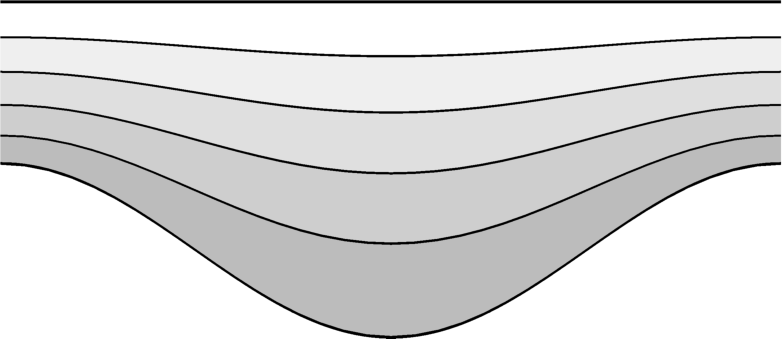
\includegraphics[width=\wgh]{a000.png}} \\
    (b, $A=0.25$ ) & (c, $A=0.5$ ) \\
    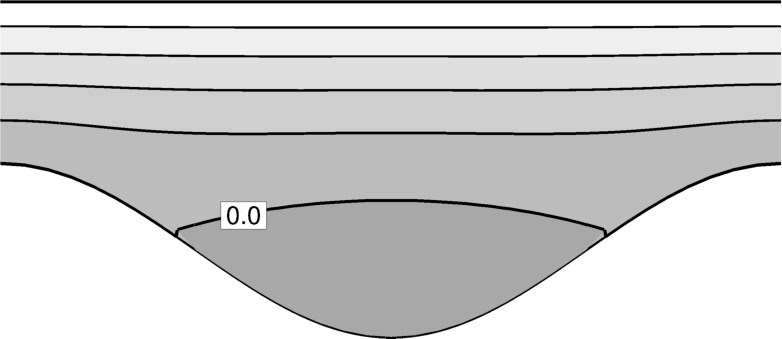
\includegraphics[width=\wgh]{a025.png}
    &
    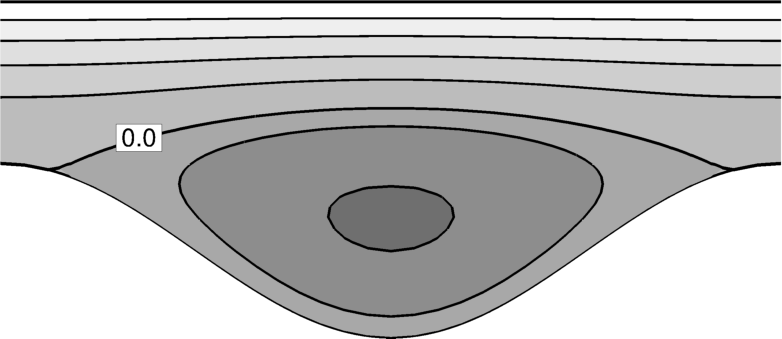
\includegraphics[width=\wgh]{a050.png} \\
    (d, $A=0.75$ ) & (e, $A=1.0$ ) \\
    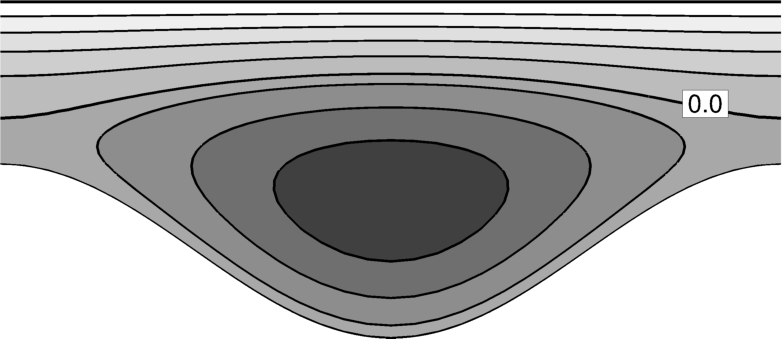
\includegraphics[width=\wgh]{a075.png}
    &
    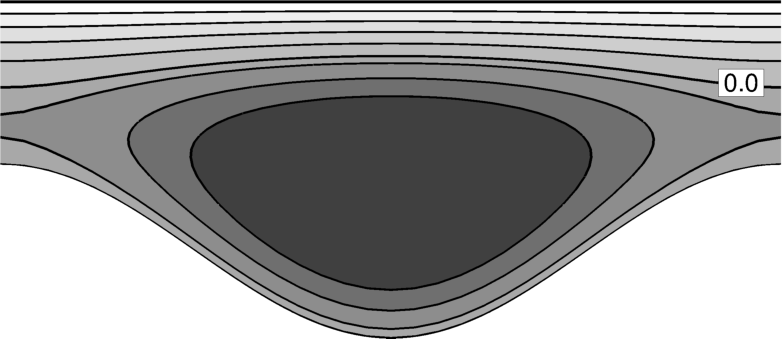
\includegraphics[width=\wgh]{a100.png} \\
    \multicolumn{2}{c}{\includegraphics[width=\textwidth]{Avar_velocity_profile.pdf}} \\
    \multicolumn{2}{c}{(f)} \\
\end{tabular}
%  
\caption{Streamwise velocity contours with changing Poiseuille pressure ratio $A$ (a-e) and streamwise velocity profiles (f) at the grove centre-line $x/\lambda_\alpha=0.5$.
Couette forcing remains unchanged and the plot shown in (a) and the left-most profile corresponds to the pure Couette action.
Distinguished contour-line corresponds to $w=0$.
Onset of the reversed flow appears first within the groove bottom. Well defined stream tube develops around $A=0.5$ and around $A<0.75$ reversed flow spans the entire wavelength.
Colour map and contour-lines same as in figure \ref{fig:streamwise_vel}.
}
 \label{fig:streamwise_prof_A}
\end{figure}

%%%%%%%%%%%%%%%%%%%%%%%%%%%%%%%%%%%%%%%%%%%%%%%%%%%%%%%%%%%%%%%%%%%
%%%%%%%%%%%%%%%%%%%%%%%%%%%%%%%%%%%%%%%%%%%%%%%%%%%%%%%%%%%%%%%%%%%

\section{Slowing down the travelling wave}\label{sec:linearStability}
Our objective here is to decrease propagation speed of the unstable travelling wave by manipulating ratio of Couette to Poiseuille forcing and if possible to decelerate or immobilize the unstable mode and the consequent,
nonlinear flow pattern that develops as the unstable mode is amplified.
We examine hydrodynamic stability by mapping the parametric space that spans the Reynolds number $Re$,
streamwise wavelength of the perturbation $\lambda_\beta = 2\pi/\beta$, determined by the size of the computational box $L_z$ and the Poiseuille pressure ratio $A$.
We use two solution methods interchangeably to perform continuation over parameters and to assure that we track the least stable mode.
First, we solve the full, nonlinear flow problem via DNS with the stationary, laminar solution as initial condition supplemented by an artificial forcing in the form of zero-mean Gaussian noise with small variance, such that the resulting perturbation remains in the linear regime and is applied only initially to excite the unstable mode.
At this stage complex amplification $\sigma$ is retrieved from the time history of the solution.
We than perform parametric continuation with the direct method solving the generalized eigenvalue problem that results from application of modal linear stability approach outlined in section \ref{sec:problemDes}, periodically verifying results using the nonlinear time-stepping used to initialize the process.
For cases where $\sigma_r\to0$, retrieving frequency with time-stepping method becomes difficult since nonlinear effects disturb the process before we are able to capture a singe periodic cycle.
In this limit we resort to the direct approach, and only $\sigma_i$ is verified against time-stepping.
Comparison of the two approaches is given in Figure \ref{fig:dns_vs_tmiestep} showing variation of $\sigma_i$ and $\sigma_r$ with $Re$ while remaining parameters remain fixed at $(\beta,A)=(0.288, 0.462)$.
Solid black line depicts results of the DNS and the dashed extension results from extrapolation of the $\sigma_r$ as $\sigma_r\to0$, while the thicker grey lines illustrate values obtained by direct solution of the eigenproblem ensuing from linearization.

\begin{figure}
\centering
	\includegraphics[width=\textwidth]{stability/figure3.pdf}
	\caption{Comparison of the time-stepping (DNS - solid black line) and direct (solution of the eigenproblem - thick grey line) methods used to recover $\sigma$ in the limit $\sigma_r\to0$. Variation of $(\sigma_r, \sigma_i)$ pair with $Re$ at $(\beta,A)=(0.288, 0.462)$. Dashed line in the left plot results from extrapolation.}
	\label{fig:dns_vs_tmiestep}
\end{figure}

For brevity of the presentation we omit various relations of parameters and present dependence of critical Reynolds number $Re_{cr}$ and phase speed $v_{p}=\sigma_r / \beta_{cr}$ ($\beta_{cr}$ represents wave number of the least attenuated perturbation) on the  Poiseuille pressure ratio $A$ and focus on the range of parameters for which $v_p\to0$.

\begin{figure}
\centering
	\includegraphics[width=0.7\textwidth]{stability/figure.pdf}  
	\caption{Variation of critical Reynolds number $Re_{cr}$ with changing Poiseuille pressure ratio $A$ for pure Poiseuille (zero wall speed - dashed line) and mixed Couette-Poiseuille (thick solid line) flow. Thick gray line corresponds to relation \eqref{eq:scale}. Dots represent conditions selected for nonlinear analysis.}
	\label{fig:recrit}
\end{figure}

We start our considerations by first looking at purely pressure driven flow, without the Couette component (zero wall speed) as this provides a direct connection to our previous studies of hydrodynamic stability and recall that in the case of pressure driven channel flow grooves result in flow destabilization \citep{Nikesh2017}.
For the geometry selected here, with grooves applied only to one of the walls and with only the Poiseuille component ($A=1$ and no Couette forcing) active the unstable mode becomes amplified already at $Re_{cr}(A=1)\approx63$.
The unstable mode has a form of a wave, with the critical wave number $\beta_{cr}=0.39$ and travels with phase speed $v_{p}={\sigma_{r}}/{\beta_{cr}}\approx0.79$ in the direction of the flow, i.e. pointed by the applied pressure (negative $z$-direction using current parametrization - see Figure \ref{fig:geom1}).
Keeping the Couette component off and decreasing the Poiseuille pressure ratio $A$ leads to a decrease in the phase speed (the unstable wave mode slows down) and increase of the critical Reynolds number.
Both quantities scale with $A$ as:
\begin{equation}
    \begin{cases}
        v_{p}(A) = v_p(A=1)\cdot A \\
        Re_{cr}(A)=Re_{cr}(A=1)/A,
    \end{cases}
    \label{eq:scale}
\end{equation}
due to the linear nature of the stability mechanism.
Consequently $Re_{cr}\to\infty$ and $v_p\to0$ as $A\to0$.
Relation \eqref{eq:scale} agrees with numerical results shown in Figures \ref{fig:recrit} and \ref{fig:phasevel}, which illustrate variation of the critical Reynolds number $Re_{cr}$ and phase speed $v_p$ with $A$, respectively.

\begin{figure}
\centering
	\includegraphics[width=0.7\textwidth]{stability/figure2.pdf}  
	\caption{Variation of phase speed of the most unstable mode $v_{p}$ at corresponding critical Reynolds (see Figure \ref{fig:recrit}) number and with changing Poiseuille pressure ratio $A$ for pure Poiseuille (zero wall speed - dashed line) and mixed Couette-Poiseuille (thick solid line) flow. Thick gray line corresponds to  relation  \eqref{eq:scale}.}
	\label{fig:phasevel}
\end{figure}

Turning the Couette component back on (speed of the moving wall is now $W=1$) we trace changes of critical conditions with variation of the Poiseuille pressure ratio parameter $A$.
Variation of the quantities of interest, i.e. critical Reynolds number and phase speed of the most unstable wave with the Poiseuille ratio $A$ are shown using thick lines in Figures \ref{fig:recrit} and \ref{fig:phasevel}.
One notes immediately that application of the Couette component has a stabilizing effect, in the sense that at $A=1$ critical Reynolds number is increased to $Re_{cr}=78$, compared to the Poiseuille only configuration and grows above $10^4$ already around $A=0.24$ (we have tested critical condition up to $Re_{cr}=13000$ at $A=0.24$).
At this point we wish to address a conjecture, stated in $\S$\ref{sec:intro}, on the possible destabilization of the Couette flow over longitudinally grooved surface.
We note that the value of Reynolds number required for the onset of unstable modes increases as $A\to0$, which indicates that without pressure forcing the flow remains stable against considered traveling wave instability up to very high (possibly arbitrary high) Reynolds numbers.
Consequently, the unstable wave mode found for the Poiseuille configuration \citep{Nikesh2017}, seems to be attenuated in the Couette configuration.
Therefore, similarly to the plane reference, Couette flow over a grooved wall remains linearly stable and nonlinear solutions are attainable only via sub-critical scenario.

Along with the stabilizing effect, application of the Couette component leads to the decrease of the phase speed of the critical perturbation. This is shown in Figure \ref{fig:phasevel}, which illustrates variation of the phase speed of the most unstable wave mode with changing of the pressure ratio.
In the $A\to1$ limit the unstable wave mode travels in the direction determined by applied pressure forcing, same as in the pure Poiseuille configuration (negative $z$-direction using current parametrization),
but with phase speed decreased due to the influence of the Couette forcing to $v_p(A=1)\approx0.3$ and at conditions corresponding to the zero bulk flow ($A=0.705)$ to $0.179$.
Further decrease of the Poiseuille pressure ratio leads to decreased phase speed and at around
$A^{*}_{cr}\approx0.462$ phase speed of the most unstable mode achieves its minimum and than again increases.
The non-monotonic change of phase speed with $A$ indicates that as the pressure gradient is decreased the unstable wave mode decelerates, eventually stops as $v_p\to0$ and than reverses for $A<A^{*}_{cr}$ and travels in the positive $z$-direction, the same as the direction of the moving wall (see also the nonlinear solutions outlined in section \ref{sec:nonlinear_saturation}).
Using bisection we estimate critical wave inversion conditions at which the most unstable mode changes direction as $v_p\to0$
to be $A^{*}_{cr}= 0.462\pm 0.0004$ and $(Re_{cr}, \beta_{cr})=(296, 0.288)$ for which $v_p=\pm10^{-6}$.

\begin{figure}
\centering
	\includegraphics[width=\textwidth]{mode-direction/figure.pdf}  
	\caption{Components of the complex amplification rate $\sigma$ at flow conditions corresponding to $Re=400$.
	Variation of $\sigma_i$ in (a) and $\sigma_r$ in (b), with streamwise length of the perturbation $\lambda_\beta=2\pi/\beta$ for a range of pressure ratios $A$ selected around $A^*(Re=400)$ for which at $Re=400$ the unstable mode changes direction and $v_p\to0$.
    Solid dots in (a) distinguish positions of maximum amplification and the thick connecting line crosses $\sigma_i=0$ line at a point where $Re_{cr}=400$, i.e. $(A_{cr}=0.427, \beta_{cr}=0.27)$, for which the unstable wave propagates in the positive $z$-direction (intersection not shown - compare with figures \ref{fig:recrit} and \ref{fig:phasevel}). Frequencies corresponding to maximal amplifications are distinguished by a thick line in (b) and travelling directions of the unstable mode are added for reference.
    For $Re=400$ pressure ratio resulting in wave reversing direction is $A^*(Re=400)=0.447$ (marked in plots with an open circle), compared to $A^*(Re_{cr})=0.462$ at critical conditions.}
	\label{fig:re400}
\end{figure}

We will now focus on the determination of pressure ratios $A^*(Re)$ corresponding to the inversion of the propagation direction of the unstable mode at conditions above critical.
To this end we test linear stability at slightly supercritical conditions and look for conditions such that for the most amplified unstable wave $\sigma_r\to0$.
Figure \ref{fig:re400} outlines the approach and shows variation of the components of the complex amplification rate $\sigma$ with streamwise perturbation wave number $\beta$ at $Re=400$ for selected values of $A$ around the wave inversion $A^{*}$ value (marked with an open circle in Figure \ref{fig:re400}a and b).
Positions corresponding to the maximum of $\sigma_i$ are marked with dots in Figure \ref{fig:re400}a and determine a curve that crosses the $\sigma_i=0$ at corresponding critical conditions (intersection not illustrated).
Corresponding values of $\sigma_r$ are distinguished by dots in Figure \ref{fig:re400}b and show that with the decrease of the pressure ratio $A$
the real part of the complex amplification $\sigma$ initially decreases to zero, determining the specific wave inversion ratio $A^*(Re)$, and than increases again as the wave changes direction.

\begin{figure}
\centering
	\includegraphics[width=0.65\textwidth]{zero-phase/figure.pdf}
	\caption{ Propagation direction of the unstable wave mode below $A^*_{cr}\approx0.462$ showing supercritical conditions for which the wave changes direction. Conditions above (below) $v_p=0$ correspond to the wave traveling in the $-z$- ($+z$)-direction. Gray region below $Re_{cr}$ line corresponds to mode attenuation. Intersection of $v_p\to0$ and $Re_{cr}(A)$ lines falls around
	$A^{*}_{cr}, Re_{cr}\approx(0.462,  296)$.
	 Dots represent conditions selected for nonlinear analysis.}
	\label{fig:zero_phase}
\end{figure}

For selected, moderately supercritical values of the Reynolds number the wave inversion ratio $A^*$ determines conditions for which phase speed of the most unstable mode decreases to the point that the unstable mode may be considered to become stationary i.e. $v_p\to0$.
This deceleration of the unstable mode is to the point that eventually this mode may be considered
a global rather than a convective instability.
We mean by that the fact, that during the amplification of such a decelerated mode spacial growth
of resulting secondary structures manifests both up- as well as down-stream in contrast to the purely convective instability which grows only downstream.
The $v_p\to0$ curve in the  $(A,Re)$ plane is shown in Figure \ref{fig:zero_phase}
and illustrates that inversion pressure ratio decreases with Reynolds number.
I.e. $A^{*}(Re>Re_{cr})<A^{*}_{cr}$.
Figure \ref{fig:zero_phase} depicts existence of distinct regions that divide the $(A,Re)$ plane.
Conditions corresponding to the region below $Re_{cr}(A)$ line (marked in gray) result in attenuation of the mode being traced.
In between the $Re_{cr}(A)$ and $v_p\to0$ curves there exist a range of parameters for which the most unstable mode is amplified, has a character of a wave propagating towards the $+z$-direction (against applied pressure), while to the right of the $v_p\to0$ line the unstable mode
travels in the $-z$ direction (along applied pressure).
The $\sigma\to0$ line distinguishes conditions for which the most unstable wave mode is immobilized and its intersection with the $Re_{cr}(A)$ curve defines critical conditions for which the unstable mode changes direction around $A^{*}_{cr}$.
% In proximity to the $\sigma\to0$ line propagation speed of the unstable mode is decreased and the nonlinear solution, that results from amplification and consequent saturation forms a slowly moving or even a standing wave solution.


%%%%%%%%%%%%%%%%%%%%%%%%%%%%%%%%%%%%%%%%%%%%%%%%%%%%%%%%%%%%%%%%%%%
%%%%%%%%%%%%%%%%%%%%%%%%%%%%%%%%%%%%%%%%%%%%%%%%%%%%%%%%%%%%%%%%%%%

\section{Nonlinear saturation of the unstable mode}
\label{sec:nonlinear_saturation}
At supercritical conditions ($Re>Re_{cr}$) small amplitude perturbations result in amplification of unstable modes.
While amplitude of the mode being amplified remains small its growth and propagation remain governed by the linear theory.
Increase of the mode's amplitude causes nonlinear interactions to become non negligible,
impeding further growth and causing the onset of the nonlinear saturation state.
For the traveling wave instability, that is considered here, the growth and transition into the nonlinear saturation state bears features of the supercritical Hopf bifurcation \citep{Nikesh2018} with the nonlinear saturation state corresponding to the system's limit cycle.
At nonlinear saturation the flow develops a number of characteristic features,
not unlike those reported for the case corrugated Poiseuille flow \citep{Nikesh2017}.
In the nonlinear solution a spanwise, periodic velocity component appears and causes the meandering like motion of the velocity tube positioned in the diverging sections of the channel accompanied by formation of pairs of counter-rotating vortices.
Both, the meandering of the velocity tube as well as vortex pairs travel through the domain at the same rate.

\begin{table}
    \centering
    \begin{tabular}{|c||c|cc||cc|cc|cc|cc|}
     \hline
    case:  & $A$ & $Re_{cr}$ & $\beta_{cr}$ & $Re$ & $\beta$ & $\sigma_i\cdot10^{3}$ & $\sigma_r\cdot10^{3}$ & $T\cdot10^{-3}$ & $T_s\cdot10^{-3}$ & $v_p\cdot10^{3}$ & direction\\ \hline
 \hline
    ~ $P_1$   & 1 & 63 & 0.385 & 100 & 0.385 & $11.9$ & $320$ & $0.02$ &1 & $833$ & $-z$ \\ 
           \hline
    $CP_1$  & 0.705 & 124 & 0.364  & 150  & 0.364 & $4.81$ & $65$  & $0.1$ & $2.4$ & $179$ & $-z$\\
    $CP_2$   & 0.462 & 296 & 0.292& 300 & 0.292 & $0.0658$ & $0.068$ &$68$ &$90$ & $0.23$ & $-z$\\
    $CP_3$   & 0.455 & 313 & 0.281 & 340 & 0.281 & $1.16$ &$10^{-5}$ & $10$ & $8$ & $<0.01$ & $-z$ \\
    $CP_4$   & 0.42 & 412 & 0.274 & 460 & 0.274 & $0.8$ & $4.4$ & $1.4$ & $15$ & $15.9$ & $+z$ \\
 \hline
    \end{tabular}
    \caption{Characterisation of the selected cases: pressure ratio, critical and applied conditions, complex amplification $\sigma$, oscillation $T$ and saturation $T_s$ times, phase speed and propagation direction of the perturbation for the cases selected for the study of saturation states. $CP$ - Couette-Poiseuille, $P$ - Poiseuille only forcing.}
    \label{tab:cases}
\end{table}

Here we discuss the transition to and character of the nonlinear saturation states using four characteristic cases outlined in Table \ref{tab:cases} and designated $CP_{1-4}$.
Each case is considered at supercritical conditions, and of special interest to us are relations of amplification and propagation rates, characterized by components of the complex amplification rate $\sigma$, during the linear stage of amplification as well as times to saturation and periods of resulting limit cycles past the nonlinear saturation.
For each of the considered cases computational boxes span two corrugation sections in the spanwise direction and correspond to respective critical perturbation wavelengths in the streamwise direction.
Consequently computational dimensions are $(L_x,L_z)=(2\lambda_\alpha, \lambda_{\beta_{cr}})$
with spanwise and streamwise periodicity assumption maintained.
For cases $CP_{1}$ and $CP_{3,4}$ applied Reynolds number range from $110\%$ to $120\%$ of respective critical values and $CP_2$ is considered at marginally supercritical conditions of about $101\%$ of the critical Reynolds number and very close to conditions determined in
section $\S$\ref{sec:linearStability} as the point where the unstable mode changes direction at the lowest value of the Reynolds number i.e. for $A\approx A^*$.
Case $CP_1$ corresponds to zero-mean base flow at $A=0.705$ and $(Re, \beta)=(150, 0.364)$ with the unstable mode travelling in the negative $z$-direction with phase speed $v_p\approx1.8\cdot10^{-1}$.
Cases $CP_2$ and $CP_3$ are particularly interesting and correspond to conditions that lie close to the $v_p\to0$ line, depicted in Figure \ref{fig:zero_phase} and feature propagation speeds of the unstable modes that are very small but with propagation in the negative $z$-direction.
Case $CP_2$ is marginally critical at $(Re, \beta)=(300, 0.292)$ and close to the intersection of $Re_{cr}(A)$ and $v_p\to0$ curves depicted in Figure \ref{fig:zero_phase}, i.e. around $A^{*}_{cr}\approx 0.462$.
Consequently this case features low phase speed of $v_p\approx2.3\cdot10^{-4}$ but also the amplification rate is moderate and small perturbation requires a long time to saturate with the resulting nonlinear state featuring a low amplitude secondary flow.
Contrary, $CP_3$ at $(Re, \beta)=(340, 0.281)$ corresponds to moderate, supercritical conditions with a relatively large amplification rate and phase speed as low as $v_p\approx10^{-5}$.
For cases $CP_{2,3}$ the amplification process, starting from small, random perturbation and up to the onset of nonlinear interactions, is illustrated in the accompanying video materials.
At this point we note, that in the $CP_2$ case, throughout the amplification stage slowly moving structures are present. This corresponds to the small, but finite phase speed of the the unstable wave traveling through the domain while it is being amplified.
In the $CP_3$ case the amplification stage is much shorter and phase speed due to the linear mechanism much lower.
Consequently developing structures remain virtually immobile throughout the amplification stage.
However, once nonlinear interactions become large enough to sufficiently change the mean flow, secondary flows begin to move and the flow settles onto a periodic cycle with a period of around $10^4$ advective time units, apparently unrelated to the linear stability result.
Finally, $CP_4$ at $A\approx0.42$ and $(Re, \beta)=(460, 0.274)$ corresponds to conditions where propagation of the unstable wave reverses towards positive $z$-direction with phase speed  $v_p\approx1.6\cdot10^{-2}$.
For comparison Table \ref{tab:cases} contains critical and stability properties at supercritical conditions (around $155\%$ of the respective $Re_{cr}$) for the travelling wave instability for the case of pure Poiseuille flow (Couette component turned of) through the considered geometry, designated as $P_1$ (compare with Figure \ref{fig:recrit}).
We note, that amplification rate is much larger for the $P_1$ case than for the $CP_{1-4}$ ($10-10^3$ times larger)
and that
at the same time phase speed of the perturbation is around $10-10^5$ times that reported for $CP_{1-4}$ cases.

\begin{figure}
\centering
	\includegraphics[width=\textwidth]{energy-plot/figure2.pdf}
	\caption{Variation of the perturbation $E_{3D}$ \eqref{eq:e3d} energy throughout saturation process for selected cases. In each case the flow is initially perturbed with an impulse of low variance Gaussian forcing (${\Var}=10^{-5}$ over $5$ time units) and left to develop into nonlinear saturation. Initial, transient stage ($t<250$) is shown on the left, and variation around saturation time $T_s\pm1000$ ($T_s$ is different for each case - see Table \ref{tab:cases}) on the right.}
	\label{fig:tstar}
\end{figure}

Each of the considered cases is started using an undisturbed, stationary flow as initial condition and low variance Gaussian forcing (${\Var}=10^{-5}$) is applied over the initial $5$ advective time units of the simulation to excite the unstable mode. Evolution of the flow is monitored using variation of the three-dimensional perturbation energy in time, defined as
\begin{equation}
E_{3D}=\frac{1}{2\Omega}\sum_{k=1}^{k=M} \int_\Omega {\bf u}_{-k}\cdot{\bf u}_kd\Omega,
\label{eq:e3d}
\end{equation}
with ${\bf u}_k(x,y)$ representing the $k$'th amplitude of the Fourier expansion \eqref{eq:modes}
and representing deviation from instantaneous spacial velocity average.
Variation of $E_{3D}$ in time is shown in Figure \ref{fig:tstar}.
For each case initial perturbation results in a brief, transient amplification-attenuation phase ($t\approx100$ - see the left part of Figure \ref{fig:tstar}) followed by a prolonged, linear amplification stage (not shown), throughout which perturbation growth is dictated by the linear mechanism.
Depending on the case, linear stage lasts in-between $10^3-10^4$ for $CP_{1,3-4}$ and up to around $10^5$ advective time units in the $CP_2$ case, depending on the perturbation amplification rate.
Eventually nonlinear interactions impede further growth and lead the flow to the nonlinear saturation state.
Using $E_{3D}$ we define saturation time $T_s$ such that $E_{3D}(t=T_s)=0.99 E_{3D}(t=T_s+1000)$
i.e. past $T_s$ perturbation energy does not change significantly with time (we tested different thresholds and time shifts, and up to reasonable values, $T_s$ does not vary much).
The right part of Figure \ref{fig:tstar} shows variation of the $E_{3D}$ around the respective saturation time $T_s$, (different for each case - see table \ref{tab:cases}).

% \begin{figure}
% \centering
% 	\includegraphics[width=\textwidth]{trajectory/figure.pdf}
% 	\caption{Projection of the velocity vector space trajectories, representing periodic behavior past saturation time $T_s$, captured at a test point $(x,y,z)=(?,?,?)$ for each of the considered case.}
% 	\label{fig:trajectory}
% \end{figure}

% We note that, since the unstable mode has a form of a wave, past $T_s$ the flow settles onto a periodic cycle with the secondary flow pattern passing periodically through the domain.
% In general, period of the cycle $T$, past nonlinear saturation corresponds to the phase speed of the amplified unstable mode.
% This is not true in the $CP_3$ case, where time-periodicity of the secondary flow deviates significantly from the value resulting from the linear approximation.
% Periodic variations of the velocity vector for all considered cases are compared by means
% of the projection of the in-plane components of the velocity vector space trajectories in Figure \ref{fig:trajectory}.
% We note that amplitude of the in-plane motions decreases in proximity of the inversion pressure ratio $A^*$ and that concurrently the time required to close the cycle increases significantly as does the period of the limit cycle.
% While changes of the in-plane motion amplitude for $CP_2$ may be partially explained by marginally supercritical conditions and amplitude of the limit cycle it is not the case for $CP_1$ and $CP_4$.
% While $CP_3$ features similar relative distance form critical conditions, lower amplification rate and longer time to saturation $T_s$ it results in larger amplitude in-plane motions and shorter oscillations period $T$ compared to $CP_2$ (see table \ref{tab:cases}).

Past saturation time $T_s$ energy of the perturbation changes little and flow topology (shown in Figures \ref{fig:topo_f141}, \ref{fig:topo_f0924}a,b and \ref{fig:topo_f084}) remains simple, limited to the passing of, possibly decelerated or reversed, periodic secondary flows through the domain.
Due to the changes in the frequency, growth rate and phase speed of the unstable mode, distance travelled by the amplified perturbation changes significantly.
Considering that the size of the prospective test domain needs to be proportional to the product of $v_p$ and $T_s$,
we note that this value is decreased from around $830$ units in the case of pure Poiseuille flow ($P_1$) to $430$ for $CP_1$, $240$ for $CP_4$, $21$ for $CP_2$, and below $0.1$ for $CP_3$.

\begin{figure}
\centering
    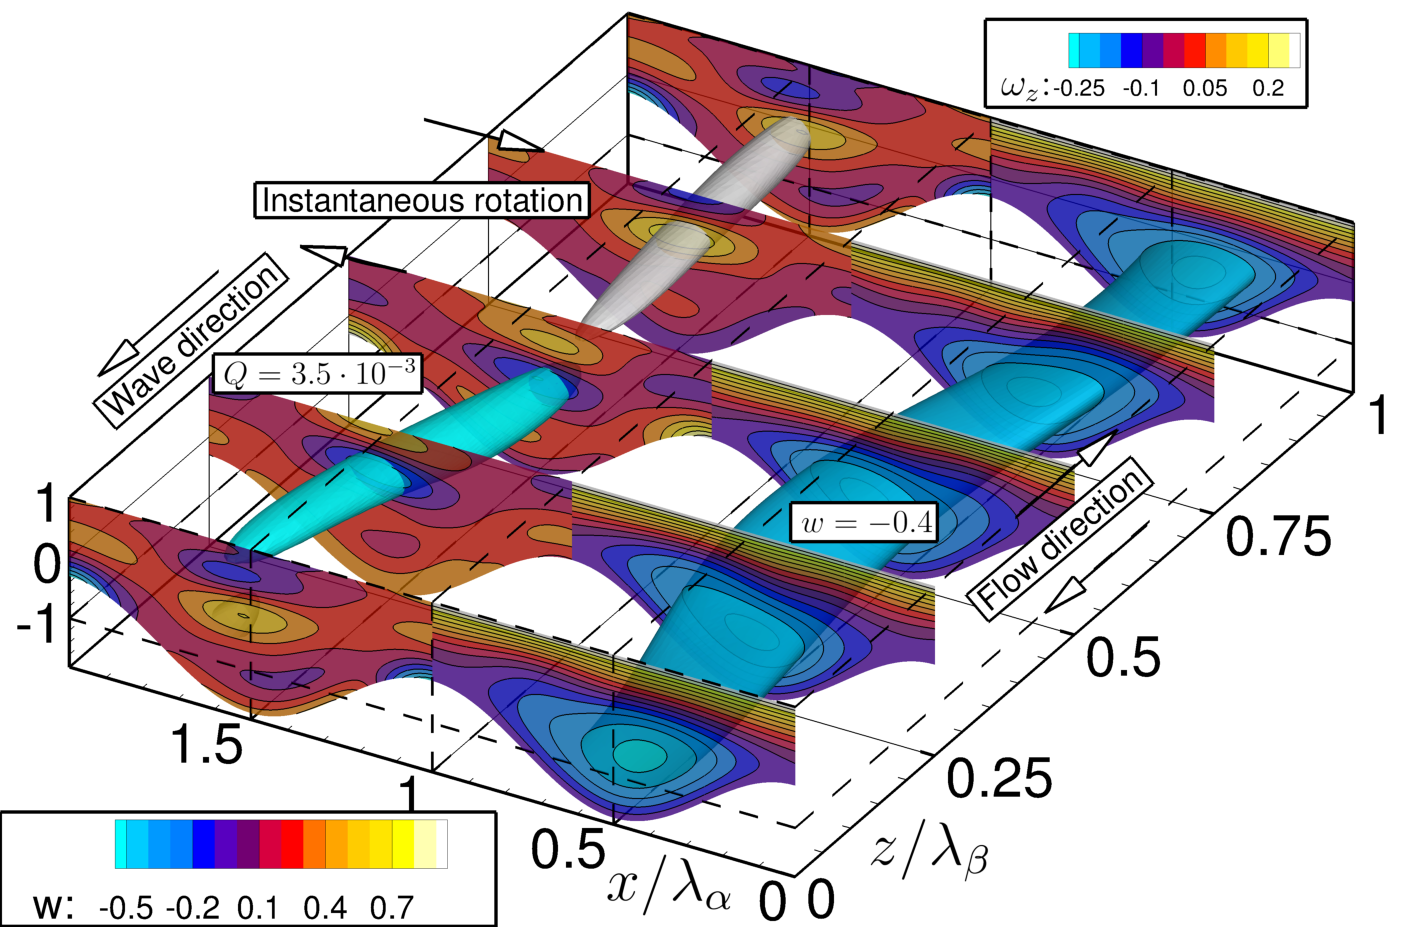
\includegraphics[width=0.75\textwidth]{f141.png}
	\caption{Snapshot of the nonstationary flow topology past the nonlinear saturation time $T_s$. Flow conditions correspond to zero-mean base flow at $A=0.705$ (case $CP_1$) and supercritical Reynolds number $Re=150$ ($Re_{cr}=124$). Length of the computational box corresponds to streamwise wave number $\beta=0.364$ ($\beta_{cr}=0.364$) and spans two corrugation sections in the spanwise direction. Slices on the right (left) depict streamwise velocity $w$ (streamwise vorticity $\omega_z$) contours. Stream tube (travelling vortex pair) is (are) shown in the right (left) part of the figure using iso-surfaces of velocity (second invariant $Q$ of the velocity gradient tensor, coloured according to the positive or negative value of streamwise vorticity $\omega_z$) taken at $w=-0.4$ ($Q=3.5\cdot10^{-3}$). Direction of the flow at the flat, top and next to the bottom walls, as well as instantaneous rotation of vortices and direction of the unstable wave propagation are marked using arrows. Phase speed of the unstable wave mode is $v_p=0.179$, with propagation direction aligned with applied pressure (negative $z$-direction).}
	\label{fig:topo_f141}
\end{figure}

At nonlinear saturation the flow develops a three-dimensional form with a number of distinctive features.
Figures \ref{fig:topo_f141} (case $CP_1$), \ref{fig:topo_f0924}a,b ($CP_2$ and $CP_3$) and \ref{fig:topo_f084} ($CP_4$) illustrate snapshots of flow topologies past nonlinear saturation time $T_s$ for each of the considered cases.
One of the distinctive changes compared to the stationary solution is onset of the meandering like motion of the streamwise velocity tubes.
This is illustrated to the right in figures by means of constant streamwise velocity surfaces (taken at $w=-0.4$ in Figure \ref{fig:topo_f141} and $w=-0.2$ in the remaining figures and velocity coloured slices.
Onset of spanwise motions is accompanied by formation of travelling vortices, illustrated by means of iso-surfaces of the second invariant $Q$ of the velocity gradient tensor, coloured by positive/negative streamwise vorticity $\omega_z$ and supplemented by arrows to indicate instantaneous rotation direction.
Qualitatively, flow solutions remain similar with the exception of the marginally supercritical $CP_2$ case, which features secondary structures of very low magnitude.

\begin{figure}
\centering
\begin{tabular}{cc}
    (a) & 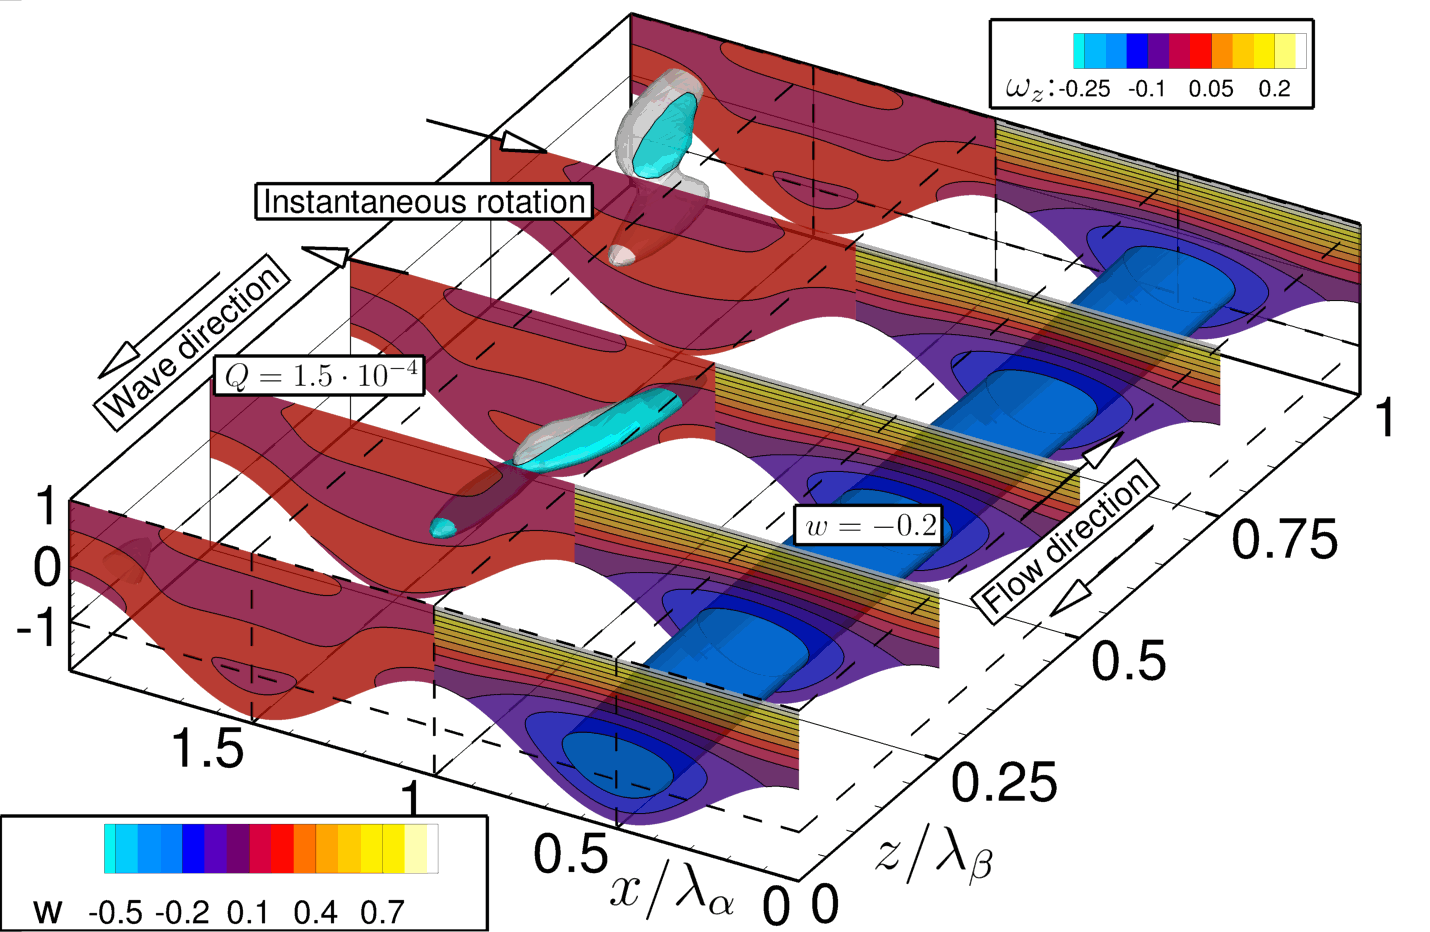
\includegraphics[width=0.75\textwidth]{f0924.png} \\
    (b) & 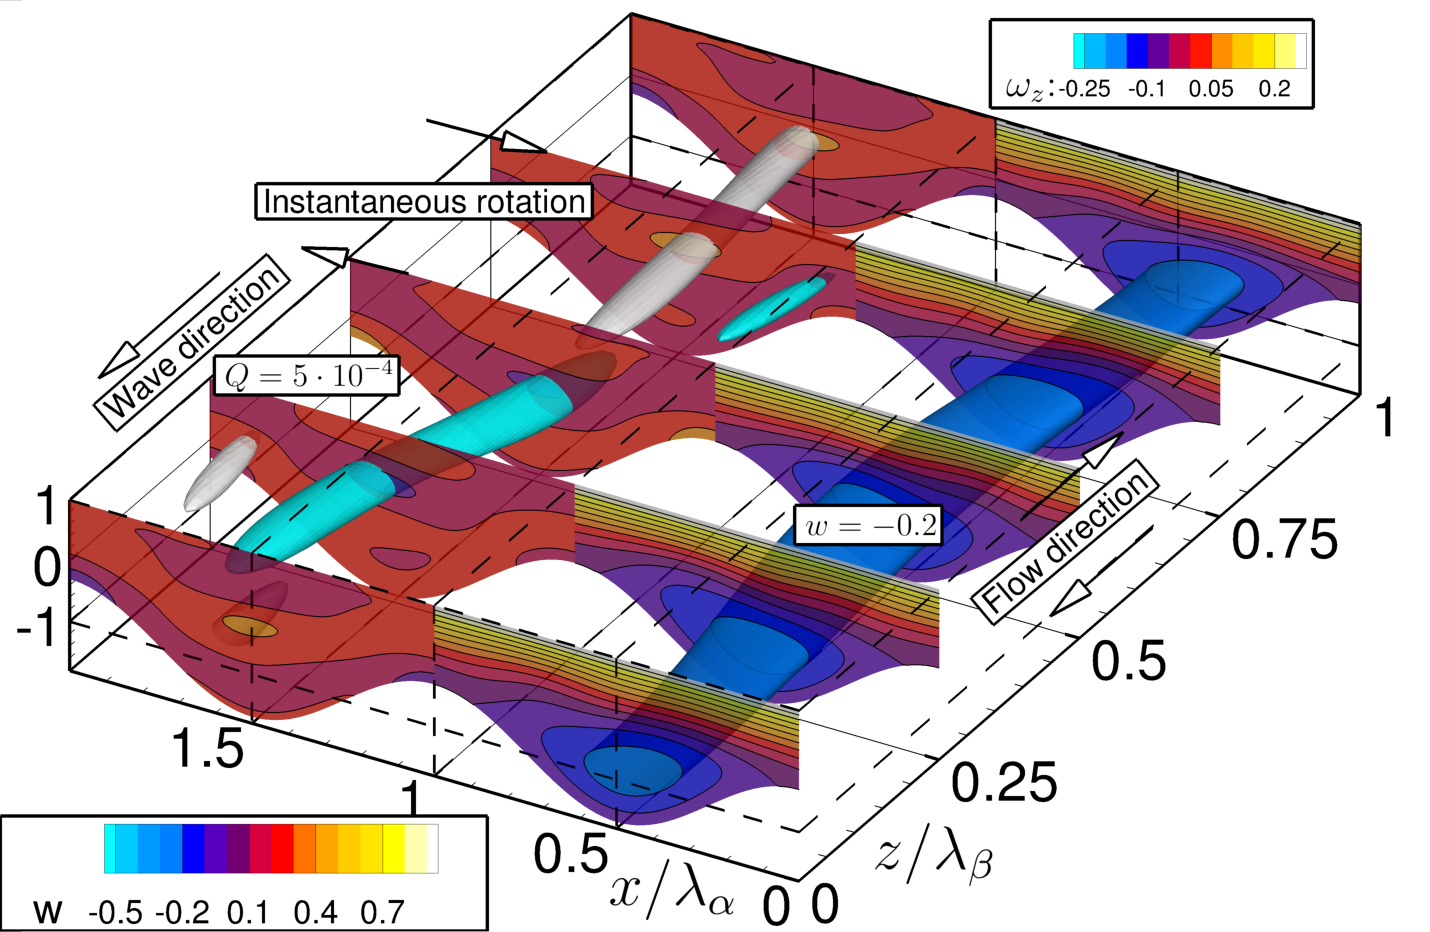
\includegraphics[width=0.75\textwidth]{f092.png} \\
\end{tabular}
\caption{Flow topology snapshots past saturation time $T_s$. Conditions chosen around $A^*$ where direction of the wave changes ($CP_{2,3}$). Respective cases correspond to $A=0.462$, $Re=300$ and $\beta=0.292$ - case $CP_2$ - $(Re_{cr}=296$, $\beta_{cr}=0.292)$ in (a)
and
$A=0.455$, $Re=340$ and $\beta=0.281$ - case $CP_3$ - ($Re_{cr}=313$, $\beta_{cr}=0.281$) in (b).
For both cases wave propagation is in negative $z$-direction.
Slices same as in Figure \ref{fig:topo_f141},
streamwise velocity iso-surfaces at $w=-0.2$ in (a,b), $Q=1.5\cdot10^{-4}$ in (a)
and $Q=5\cdot10^{-4}$ in (b).}
\label{fig:topo_f0924}
\end{figure}

\begin{figure}
\centering
    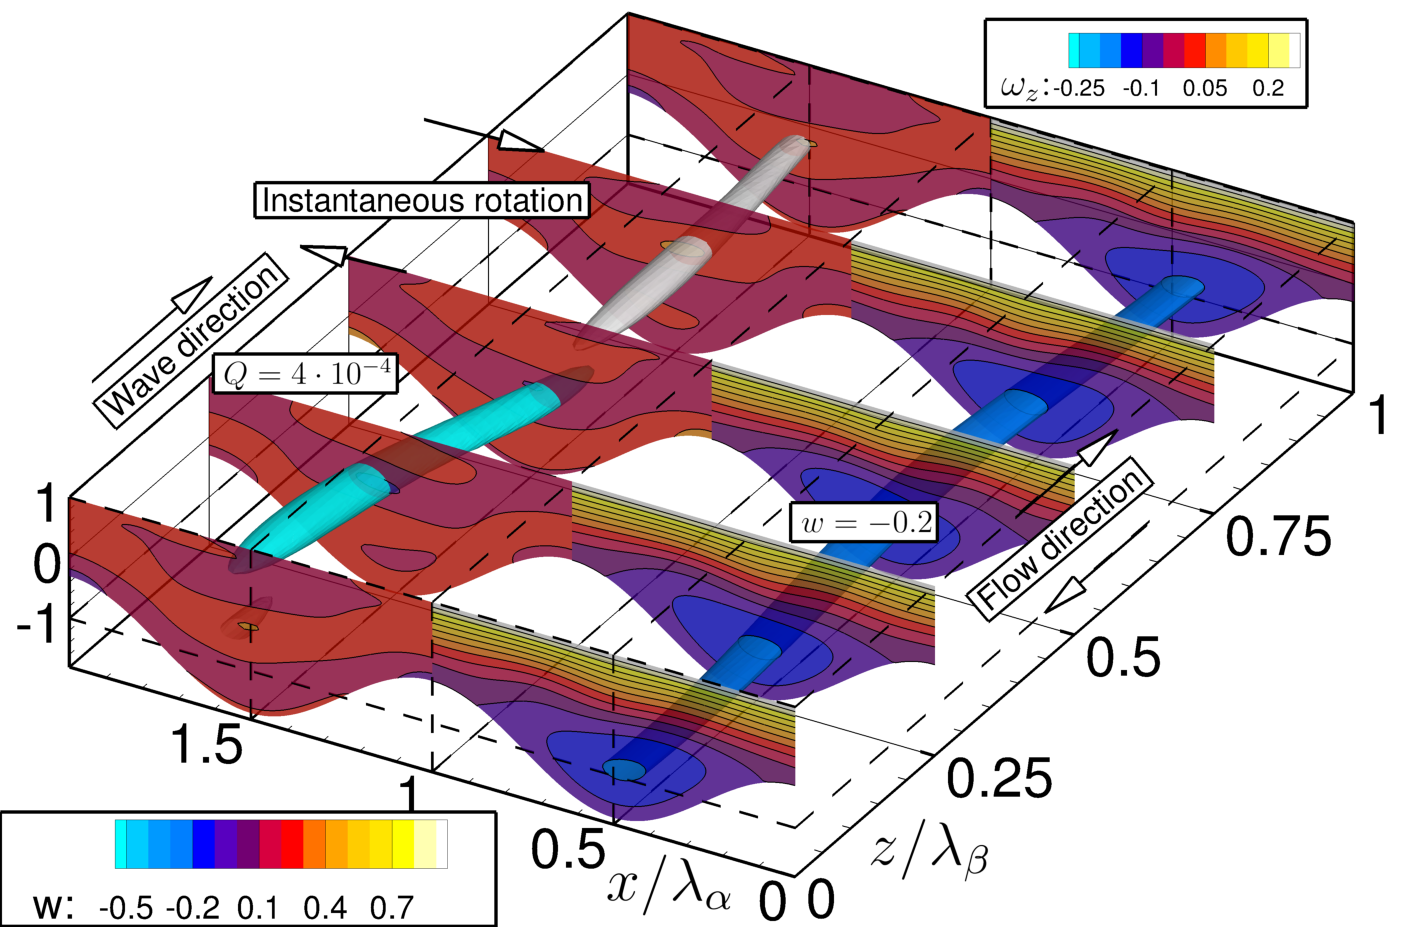
\includegraphics[width=0.75\textwidth]{f084.png}
	\caption{Flow topology snapshot past saturation time $T_s$. Conditions are
$A=0.42$, $Re=460$ and $\beta=0.27$ (case $CP_4$, $Re_{cr}=412$, $\beta_{cr}=0.274$) with the unstable wave changing direction and propagating against applied pressure (positive $z$-direction).
Slices same as in Figure \ref{fig:topo_f141},
streamwise velocity iso-surfaces at $w=-0.2$ and $Q=4\cdot10^{-4}$.}
	\label{fig:topo_f084}
\end{figure}

In the case of corrugated channel flow with only the Poiseuille forcing applied \citep{Nikesh2017,Nikesh2021} flow features formed in consequence of nonlinear saturation propagate downstream, along the direction that the applied pressure acts.
In the case of the $CP$ configuration, considered here propagation direction might change as the Poiseuille component is decreased.
Features formed as a result of nonlinear saturation of cases $CP_{1-3}$ propagate in the negative $z$-direction, marked in in figures using arrows.
Case $CP_4$ corresponds to conditions where the unstable mode, and consequently three-dimensional features of the saturated flow propagate against the pressure, i.e. the positive $z$-direction.

\begin{figure}
\centering
\begin{tabular}{cc}
    (a) & 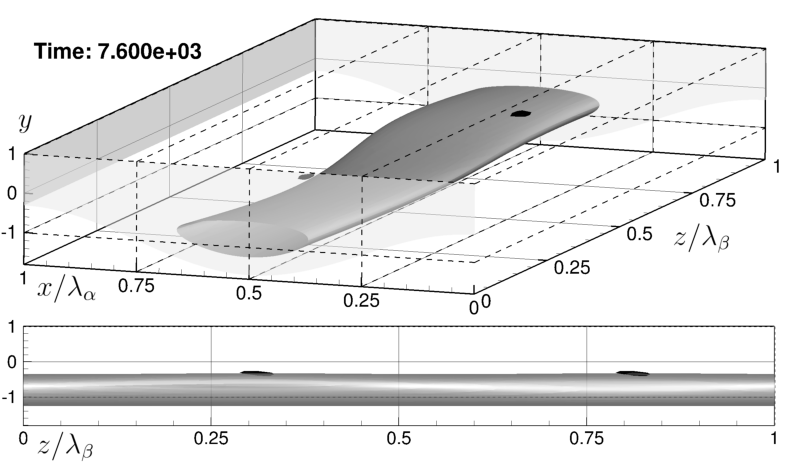
\includegraphics[width=0.75\textwidth]{f092_7600.png} \\
    (b) & 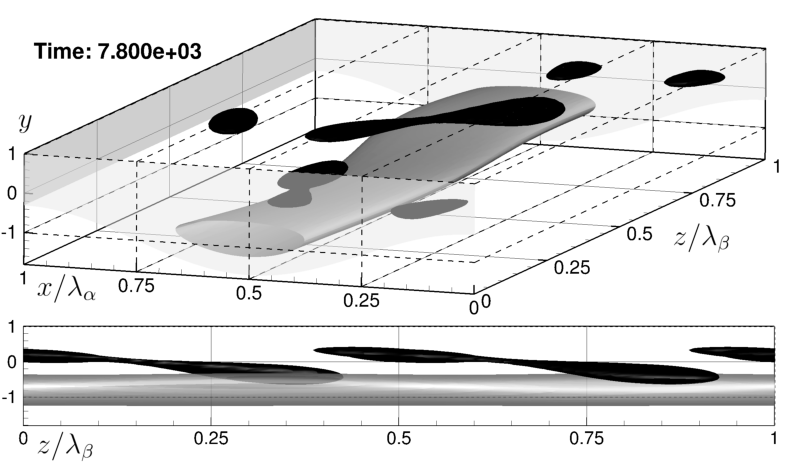
\includegraphics[width=0.75\textwidth]{f092_7800.png} \\
    (c) & 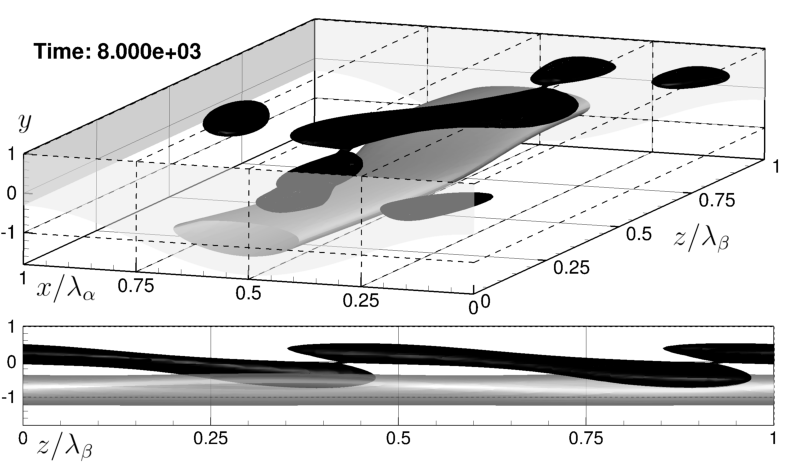
\includegraphics[width=0.75\textwidth]{f092_8000.png} \\
\end{tabular}
\caption{Iso-surfaces of the streamwise velocity component at $w=0.2$ (gray) and second invariant $Q$ of the velocity gradient tensor at $Q=4\cdot10^{-4}$ at times close to the saturation time $T_s$
for the $CP_3$ case at $t=7.6\cdot10^3$ (a), $t=7.8\cdot10^3$ (b) and $t=8\cdot10^3$ (c) illustrating both up- and down-stream propagation of the secondary flow structure.} 
\label{fig:topo_092_time}
\end{figure}

We now focus on $CP_2$ and especially $CP_3$ cases, which we consider to be especially interesting since for those cases propagation speed of the unstable wave decreases substantially.
Amplification process, starting with the initial random perturbation and past the nonlinear saturation, captured for those cases is illustrated in the accompanying video materials.
In the case of $CP_2$, due to the low value of the Reynolds number amplification rate remains small, leading to a long time that is required for the nonlinear saturation to take place and allowing for the observation of the amplification phase for around $2\times10^5$ advective time units.
It is interesting to point out that, while formally the unstable mode remains a traveling wave and instability itself, a convective one, the time that it takes for the wave to pass through the computational domain, i.e. travel a single perturbation wavelength is around $6.8\times10^4$ time units.
At the same time nonlinear effects, such as noticeable bending of the velocity tube and onset of vortex pairs, while small in amplitude due to marginal supercriticality of the case, become noticeable already around $9\times10^4$ time units (wave travels less than $1.5$ perturbation wavelengths) and
throughout the entire process shown in the video the wave travels a distance of roughly three times the length of the computational box.
On the other hand, very low phase speed obtained for the unstable mode in the $CP_3$ case results in virtually no movement of the unstable mode during amplification (travelled distance is below $0.1$ length units).
Consequently, throughout the amplification stage the unstable mode may be considered stationary, with resulting secondary flow structures developing both up- and down-stream.
Therefore, in the qualitative sense considered instability becomes global.
Figure \ref{fig:topo_092_time} illustrates this by depicting changes to the flow field at selected time instances close to the saturation time $T_s$ taken every $200$ time units.
Immobility of the developing secondary flow structure is illustrated by the streamwise velocity component iso-surface at $w=0.2$, which shows developed but motionless meandering pattern formed in the diverging section of the channel. 
At the same time spatial growth of the immobilized secondary flow is illustrated with iso-surfaces of the second velocity gradient tensor invariant $Q$,
showing spatial spread of flow regions where features of the secondary flow develop.
It should be noted that spacial growth runs both in the positive as well as negative $z$-direction  and developing structures are not advected by the bulk of the flow indicating a global, rather than convective character of the process, at least prior to saturation.
Finally we note that past the saturation time, possibly due to the changes to the mean flow by the nonlinear mechanism, developed secondary flow structures begin moving in the direction pointed by applied pressure and the flow settles onto a periodic cycle solution. 

% \begin{figure}
% \centering
% 	\includegraphics[width=0.7\textwidth]{sat-shear/figure.pdf}
% 	\caption{Variation of the rate of strain averaged over the streamwise direction \eqref{eq:gamma_streamwise_avg} at the moving plane wall, throughout nonlinear saturation process, along the spanwise $x$-direction across a single corrugation wavelength $\lambda_\alpha$. Flow conditions correspond to case $CP_1$, pressure ratio $A=0.705$ at $Re=150$ ($Re_{cr}=124$). Line colour saturation is proportional to the advancement of time from laminar towards saturation state, with light grey depicting the state at $t=0.1T_s$ up to solid black at $T_s$. Compare with rate of strain for stationary solution at $A=0.75$ shown in Figure \ref{fig:rate_of_strain}.}
% 	\label{fig:satruration_rate_of_strain}
% \end{figure}

% We conclude description of the nonlinear saturation states by focusing on the variation of the rate of strain $\gamma$, proportional to the drag force, exerted on the moving wall throughout saturation.
% This variation is shown in Figure \ref{fig:rate_of_strain} for the stationary base flow.
% At saturation the flow exhibits spatial and temporal periodicity and we will consider distribution of the rate of strain along the spanwise direction and averaged over the streamwise direction, defined as:
% \begin{equation}
% \left.\overline{\gamma(x)}\right|_{0}^{\lambda_{\beta}}=
% 1/\lambda_\beta \int_{z=0}^{\lambda_\beta} \frac{dw}{dy}|_{y=1} dz.
%     \label{eq:gamma_streamwise_avg}
% \end{equation}
% Figure \ref{fig:satruration_rate_of_strain} shows changes of the streamwise averaged rate of strain throughout the saturation process for case $CP_1$ ($A=0.705$).
% We note that at the initial stages the rate of strain attains maximum in the diverging and minimum in the converging sections.
% As the flow transitions a local minimum forms directly above the groove center.
% Overall rate of strain increases from $\gamma_{mean} = 1.72$ for the stationary flow to $\gamma_{mean} = 1.91$ at saturation (compare with Figure \ref{fig:flowRate_avgStrain}).

%%%%%%%%%%%%%%%%%%%%%%%%%%%%%%%%%%%%%%%%%%%%%%%%%%%%%%%%%%%%%%%%%%%
%%%%%%%%%%%%%%%%%%%%%%%%%%%%%%%%%%%%%%%%%%%%%%%%%%%%%%%%%%%%%%%%%%%

\section{Conclusion} \label{sec:conclusion}
Study of a Couette-Poiseuille flow through a channel with the flat driving, and corrugated stationary wall with an opposing pressure gradient has been performed.
The primary reason for this research lies in establishing flow conditions that lead to the onset of low-Reynolds number hydrodynamic instabilities, in the form of travelling waves and at the same time allow for drastic decrease of propagation speeds and distances traveled by those waves, down to the point that timescales associated with wave amplification and propagation may be considered to decouple and the instability itself global, rather than convective.

We have characterized main properties of the two-dimensional, stationary flow for the selected geometry which offers destabilization at very low values of the Reynolds number ($Re_{cr}<10^2$).
Using smooth CP flow as reference, we illustrate properties of the flow for a range of Couette to Poiseuille ratios and discuss formation of distinct flow features in the stationary regime.

The analysis shows that addition of the Couette component decreases phase speed of the perturbation but also has a stabilizing effect, compared to the pressure only driven flow.
Our results suggests that decreasing the pressure gradient down to the limit of Couette only forcing causes the flow through the corrugated geometry to become unconditionally stable, similarly to the classical plane wall Couette flow.

The nonlinear analysis performed for selected cases corresponding to zero-mean and close to minimum phase speed conditions illustrates a possibility for orders of magnitude reduction in the perturbation propagation speed compared to the pure Poiseuille configuration (see Table \ref{tab:cases}).
Presented results suggest significant reduction of the distance traveled by the amplified perturbation and in some of the cases, immobilization of the unstable mode during linear amplification phase.

Using data from Table \ref{tab:cases}, saturation time $T_s$ and phase speed one can attempt to estimate distances covered by the travelling wave mode as it grows during the linear amplification stage.
For the case $CP_2$ distance travelled by the perturbation is reduced to around $20$ units, distance comparable to perturbation wavelength and for $CP_3$ this is below $0.1$ units,
indicating that the unstable mode becomes virtually immobile.
By comparison, in the case of the pure Poiseuille forcing this distance is close to $900$ units or $50$ perturbation wavelengths.

%%%%%%%%%%%%%%%%%%%%%%%%%%%%%%%%%%%%%%%%%%%%%%%%%%%%%%%%%%%%%%%%%%%
%%%%%%%%%%%%%%%%%%%%%%%%%%%%%%%%%%%%%%%%%%%%%%%%%%%%%%%%%%%%%%%%%%%

\section*{Acknowledgement}
We thank prof. J. M. Floryan (University of Western Ontario) for interesting discussions that have led us to a number of ideas concerning flows through corrugated passages as well as Łukasz Klotz and Tomasz Bobiński (Warsaw University of Technology) for valuable discussions on the possible experimental set-up configuration.
Authors also acknowledge financial support of the National Science Centre, Poland in the form of Preludium-15 (2018/29/N/ST8/00846) and Sonata-15 (2019/35/D/ST8/00090) grants.
Numerical computations were performed at the computing facilities of the Aerodynamics Division at the Faculty of Power and Aeronautical Engineering of Warsaw University of Technology.

%%%%%%%%%%%%%%%%%%%%%%%%%%%%%%%%%%%%%%%%%%%%%%%%%%%%%%%%%%%%%%%%%%%
%%%%%%%%%%%%%%%%%%%%%%%%%%%%%%%%%%%%%%%%%%%%%%%%%%%%%%%%%%%%%%%%%%%

\section*{Declaration of Interests}
The authors report no conflict of interest.

\section*{Data Availability}
The data that support the findings of this study are available from the corresponding author upon reasonable request.

%%%%%%%%%%%%%%%%%%%%%%%%%%%%%%%%%%%%%%%%%%%%%%%%%%%%%%%%%%%%%%%%%%%
%%%%%%%%%%%%%%%%%%%%%%%%%%%%%%%%%%%%%%%%%%%%%%%%%%%%%%%%%%%%%%%%%%%

\section*{Appendix}
\label{appendix}
Accuracy of the computational method is asserted
through grid convergence study.
We compare values of the complex amplification rate
$\sigma=\sigma_r+i\sigma_i$ obtained
using a set of meshes of increasing complexity and 
varying the degree of elemental polynomial expansion.
The case considered here corresponds to the laminar zero mean flow, $A=0.705$.
Results obtained using the largest mesh of $15\times13$
quadrilaterals combined with up to $7$'th order polynomials are used
as reference. Analysis of the results presented in Table
I shows that acceptable accuracy is achievable using a
grid consisting of $13\times11$ quadrilaterals in combination with up to fifth order
polynomial expansion.

 \begin{table}
     \centering
\begin{tabular}{|c|c|c|c|c|c|}
\hline 
 {Elements}        & Oder    & $\sigma_{i}\cdot10^{2}$      &  $\sigma_{r}\cdot10^{2}$ &  $\epsilon_{\sigma_i}$   & $\epsilon_{\sigma_r}$   

                        
\\ \hline
                             & 3    & $4.825$      & $6.500$  &  $1.7e^{-5}$  & $1.1e^{-6}$
\\ \cline{2-6}
                $9 \times11$ & 5    & $4.817$      & $6.501$  &  $3.57e^{-8}$  & $2.2e^{-9}$
\\ \cline{2-6} 
                             & 7    & $4.817$      & $6.501$  &  $2.34e^{-8}$  & $1.12e^{-9}$
\\ \hline



                            & 3    & $4.821$      & $6.502$  &  $1.15e^{-6}$  & $2.2e^{-7}$
\\ \cline{2-6}
\rowcolor{Gray}
                $13\times11$   & 5    & $4.817$      & $6.502$  &  $7.34e^{-9}$  & $1.05e^{-9}$ 
\\ \cline{2-6} 
                              & 7    & $4.817$      & $6.501$  &  $2.8e^{-9}$  & $1.19e^{-9}$
\\ \hline
                            & 3    & $4.816$      & $6.502$  &  $1.17e^{-6}$  & $2.34e^{-7}$
\\ \cline{2-6}
                $15\times13$ & 5    & $4.817$      & $6.501$  &  $7.1e^{-9}$  & $8.8e^{-10}$ 
\\ \cline{2-6} 
                              & 7    & $4.817$      & $6.501$  &  $-$  & $-$
\\ \hline
\end{tabular}
\caption{Grid convergence for the computation of the complex amplification rate $\sigma$ of the least stable mode using a sequence of meshes and polynomial expansions. Conditions correspond to $A=0.705$, $Re=150$ and $\beta=0.36$. Selected configuration marked with grey.}
\label{tab:tab1}
\end{table}

% Time stepping (DNS) and direct solution of the eigenproblem resulting from linearization have been used in the parametric continuation study of hydrodynamic stability. Figure \ref{fig:dns_vs_tmiestep} compares values of the complex amplification rate $\sigma$ calculated for $A=?$. With the reduction of the Reynolds number  $\sigma_r\to0$ and tracking temporal variations with the time-stepping method becomes difficult. Amplification rate $\sigma_i$ is recovered with both methods.

% Note the spaces between the initials
\bibliographystyle{jfm}
% Note the spaces between the initials
\bibliography{paper}

\end{document}
